\documentclass[11pt,a4paper,openany]{book}
\usepackage[T2A]{fontenc}
\usepackage[utf8]{inputenc}
\usepackage[english,russian]{babel}
\usepackage{amsmath,amssymb,mathtools,bm}
\usepackage{graphicx}
\usepackage{booktabs,array,multirow,tabularx}
\usepackage[dvipsnames]{xcolor}
\usepackage[most]{tcolorbox}
\usepackage{enumitem}
\usepackage[font=small,labelfont={bf,color=ink},textfont={color=sub},margin=0.5cm]{caption}
\usepackage[a4paper,top=2.3cm,bottom=2.4cm,left=2.4cm,right=2.4cm,headheight=14pt]{geometry}
\usepackage{fancyhdr}
\usepackage{titlesec}
\usepackage{microtype}
\usepackage[colorlinks=true,linkcolor=circ,urlcolor=circ,citecolor=circ]{hyperref}

\graphicspath{{figs/}}

% цвета — те же, что в рисунках
\definecolor{ink}{HTML}{1D1D1F}
\definecolor{sub}{HTML}{5F6368}
\definecolor{dim}{HTML}{9AA0A6}
\definecolor{faint}{HTML}{EEF0F2}
\definecolor{circ}{HTML}{2A6FDB}
\definecolor{rad}{HTML}{D93A3A}
\definecolor{load}{HTML}{D18B00}
\definecolor{plast}{HTML}{7B4EA3}
\definecolor{hydr}{HTML}{1E9E6A}
\color{ink}

% заголовки в духе 3Blue1Brown: крупно, просто, цветная полоска
\titleformat{\chapter}[display]
  {\normalfont\color{ink}}
  {\color{circ}\large\scshape Глава \thechapter}
  {6pt}
  {\Huge\bfseries}
  [\vspace{4pt}{\color{circ}\titlerule[1.2pt]}]
\titlespacing*{\chapter}{0pt}{-10pt}{22pt}
\titleformat{\section}{\normalfont\Large\bfseries\color{ink}}{\color{circ}\thesection}{0.8em}{}
\titleformat{\subsection}{\normalfont\large\bfseries\color{ink}}{\color{sub}\thesubsection}{0.8em}{}

\pagestyle{fancy}
\fancyhf{}
\fancyhead[LE]{\small\color{sub}\leftmark}
\fancyhead[RO]{\small\color{sub}\rightmark}
\fancyfoot[C]{\small\color{sub}\thepage}
\renewcommand{\headrulewidth}{0pt}

\setlist{itemsep=2pt,topsep=4pt}
\setlength{\parskip}{3pt}

% блоки
\newtcolorbox{idea}[1][Интуиция]{enhanced,breakable,colback=circ!5,colframe=circ,boxrule=0pt,leftrule=3pt,arc=0pt,
  title={#1},fonttitle=\bfseries\color{circ},coltitle=circ,colbacktitle=circ!5,attach title to upper={\ ---\ },
  left=8pt,right=8pt,top=6pt,bottom=6pt}
\newtcolorbox{keyf}[1][Главная формула]{enhanced,colback=white,colframe=load,boxrule=1.2pt,arc=4pt,
  title={#1},fonttitle=\bfseries\small,coltitle=white,colbacktitle=load,left=8pt,right=8pt}
\newtcolorbox{warnbox}[1][Ограничение]{enhanced,breakable,colback=rad!4,colframe=rad,boxrule=0pt,leftrule=3pt,arc=0pt,
  title={#1},fonttitle=\bfseries\color{rad},coltitle=rad,colbacktitle=rad!4,attach title to upper={\ ---\ },left=8pt,right=8pt}
\newtcolorbox{codebox}{enhanced,breakable,colback=faint,colframe=faint,boxrule=0pt,arc=3pt,left=8pt,right=8pt,
  fontupper=\small\color{sub}}
\newcounter{ex}[chapter]
\renewcommand{\theex}{\thechapter.\arabic{ex}}
\newtcolorbox{exercise}{enhanced,breakable,colback=hydr!4,colframe=hydr,boxrule=0pt,leftrule=3pt,arc=0pt,
  before upper={\refstepcounter{ex}\textbf{\color{hydr}Упражнение \theex.}\ },left=8pt,right=8pt}

\newcommand{\code}[1]{\texttt{\small #1}}
\newcommand{\fig}[3][0.98]{\begin{figure}[htbp]\centering\includegraphics[width=#1\linewidth]{#2}\caption{#3}\label{fig:#2}\end{figure}}
\newcommand{\eps}{\varepsilon}
\newcommand{\TSSD}{\mathrm{TSSD}}
\newcommand{\TSSP}{\mathrm{TSSP}}
\newcommand{\RHF}{\mathrm{RHF}}

\hypersetup{pdftitle={Модель гидридов в оболочках из циркония: учебник},pdfauthor={ring-tests/hydrides}}

\begin{document}
\frontmatter
\begin{titlepage}
\centering
\vspace*{2.2cm}
{\color{circ}\rule{\linewidth}{1.5pt}}\\[14pt]
{\Huge\bfseries Как гидриды выбирают\\[6pt] направление}\\[12pt]
{\Large\color{sub} Учебник по клеточно-кинетической модели гидридов\\ в трубах из циркониевых сплавов}\\[10pt]
{\color{circ}\rule{\linewidth}{1.5pt}}\\[1.2cm]
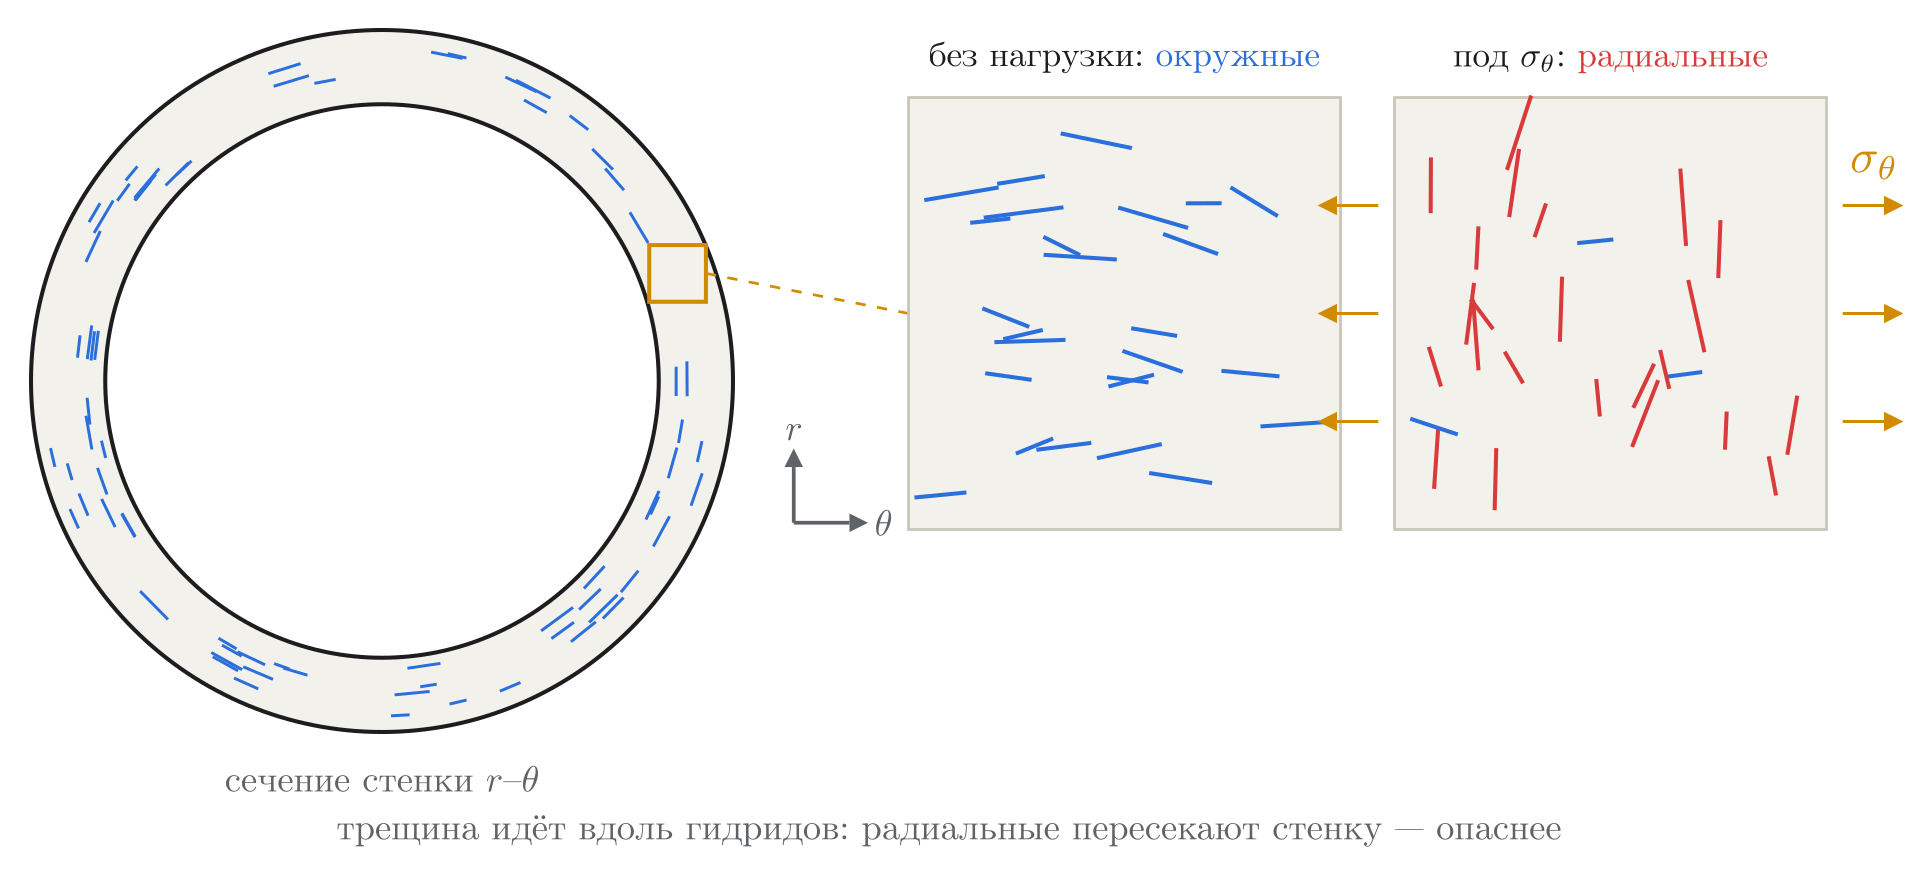
\includegraphics[width=0.9\linewidth]{F01_Tube}\\[1.2cm]
{\large Для тех, кто хочет понять модель с карандашом в руке:\\ физика, уравнения, постановки, алгоритм, проверки, границы}\\[2.4cm]
{\color{sub} Проект \texttt{ring-tests/hydrides}\quad·\quad октябрь 2026}
\end{titlepage}

\chapter*{Как читать эту книгу}
\addcontentsline{toc}{chapter}{Как читать эту книгу}

Эта книга объясняет одну модель: как при остывании трубы из циркониевого сплава в ней
выпадают пластинки гидрида и почему они ложатся вдоль окружности или поперёк неё, по радиусу.
Модель собиралась по шагам в течение нескольких сессий работы; здесь она изложена целиком,
от физики до кода, в том виде, в каком она есть сейчас, вместе с тем, что в ней не работает.

\paragraph{Три слоя.} Каждая глава построена одинаково.
\begin{enumerate}
\item \textbf{Картинка и интуиция.} Сначала --- что происходит, на пальцах и на рисунке.
  Синие блоки «Интуиция» можно читать отдельно от остального текста: из них складывается
  короткий рассказ о модели.
\item \textbf{Уравнения.} Затем --- формулы, откуда они берутся и что в них означает каждая буква.
  Главные формулы обведены золотой рамкой.
\item \textbf{Упражнения.} Зелёные блоки --- задачи, которые стоит решить на бумаге. Большинство
  решается за 5--15 минут с калькулятором; ответы и решения --- в приложении~\ref{app:answers}.
  Это не проверка, а способ «потрогать» числа: после них станет понятно, почему градус
  температуры важнее сотни мегапаскалей и почему пластичность нельзя выбросить.
\end{enumerate}
Красные блоки «Ограничение» честно говорят, где модель упрощает или где она пока не сходится
с опытом. Серые блоки «Где в коде» указывают файлы в папке \code{hydrides/automaton}.

\paragraph{Что нужно знать заранее.} Производные и интегралы, экспонента и логарифм, немного
линейной алгебры (матрицы $2\times2$, собственные векторы). Тензоры напряжений и деформаций
вводятся в главе~\ref{ch:misfit} с нуля, в объёме, нужном для модели. Преобразование Фурье
объясняется там же на одном примере.

\paragraph{Карта.} Рисунок~\ref{fig:F02_Map} --- оглавление в картинке: какие блоки есть в модели,
что они передают друг другу и в какой главе разобран каждый. Модель принимает на вход
\emph{условия опыта} (сплав, текстуру, водород, температурную историю, нагрузку) и выдаёт
\emph{структуру} гидридов и её меры, которые сравниваются с шлифами.

\fig{F02_Map}{Модель целиком. Внутри клеточного автомата четыре физических блока обмениваются
данными на каждом шаге по времени; новые пластинки меняют и поле напряжений, и водород вокруг.}

\paragraph{Обозначения.} Окружное направление трубы обозначается $\theta$ (оно же TD в
металлографии), радиальное --- $r$ (ND), осевое --- $z$ (RD). На всех рисунках
\textcolor{circ}{окружные} гидриды синие, \textcolor{rad}{радиальные} --- красные, нагрузка
\textcolor{load}{золотая}, пластичность \textcolor{plast}{фиолетовая}, водород \textcolor{hydr}{зелёный}.
Полный список обозначений и параметров --- в приложении~\ref{app:ref}.

\tableofcontents

\mainmatter
\chapter{Задача: гидриды в стенке трубы}\label{ch:problem}

\section{Откуда в трубе гидриды}

Оболочки твэлов и направляющие каналы тепловыделяющих сборок делают из сплавов циркония:
Zircaloy-4, Zr--1Nb, Э110, Э635 (Zr--Nb--Sn--Fe). В реакторе цирконий окисляется водой, и часть
водорода, освободившегося при коррозии, уходит в металл. При рабочей температуре водород
растворён, но растворимость быстро падает с температурой: при 400\,$^\circ$C металл держит
около 170 частей на миллион по массе (ppm), при комнатной --- меньше одной. Всё лишнее при
остывании выпадает в виде \emph{гидрида} --- отдельной фазы $\delta$-ZrH$_{1.66}$, у которой
на атом циркония приходится 1.66 атома водорода.

Гидрид выпадает тонкими пластинками: толщина --- доли микрона, длина --- единицы--десятки
микрон. Он хрупкий, и трещина охотно идёт вдоль пластинок. Поэтому важно, \emph{как они лежат}.

\fig{F01_Tube}{Слева --- сечение трубы. В нём пластинки гидрида обычно лежат вдоль окружности
(синие). Если труба остывает под окружным напряжением $\sigma_\theta$ (внутреннее давление),
новые пластинки могут лечь по радиусу (красные). Такие гидриды выстраиваются поперёк стенки и
опасны: трещине почти не нужно идти по металлу.}

\begin{idea}
Окружные гидриды лежат «вдоль слоёв» стенки, и трещина, идущая изнутри наружу, вынуждена
пересекать их по одному. Радиальные гидриды лежат поперёк стенки --- по пути трещины. Поэтому
переориентация гидридов под нагрузкой --- главный вопрос при сухом хранении отработавшего
топлива и при испытаниях колец, которыми занимается проект.
\end{idea}

\section{Кристалл, текстура и почему гидриды обычно окружные}

Цирконий --- гексагональный металл. У каждого зерна есть ось $c$ и перпендикулярная ей
\emph{базисная} плоскость. Гидрид выпадает пластинкой почти параллельно базисной плоскости
(точнее, на плоскостях типа $\{10\bar17\}$, в $14.7^\circ$ от базиса). Значит, ориентацию
пластинки задаёт ориентация зерна.

При прокатке трубы зёрна поворачиваются так, что оси $c$ смотрят в основном по радиусу с наклоном
$\pm\chi_0\approx 30$--$40^\circ$ к окружности. Это \emph{текстура}, и её обычно описывают
факторами Кернса $f_r$, $f_\theta$, $f_z$ --- средними квадратами косинусов оси $c$ с тремя
направлениями ($f_r+f_\theta+f_z=1$). У листа Zircaloy-4 из опытов Lepine $f_r\approx0.59$,
$f_\theta\approx0.30$, $f_z\approx0.12$.

Если ось $c$ смотрит почти по радиусу, базисная плоскость --- а с ней и пластинка --- лежит почти
по окружности. Отсюда окружные гидриды «по умолчанию». Чтобы получить радиальный гидрид, нужно
либо зерно с осью $c$ по окружности (таких меньшинство), либо механизм, который выстраивает
пластинки в радиальную цепочку. Оба пути есть в модели; второй, коллективный, оказался
важнее, чем казалось (гл.~\ref{ch:results}).

\begin{exercise}
Проверьте связь факторов Кернса с наклоном. Пусть оси $c$ лежат в плоскости $r$--$\theta$ под
углом $\chi$ к радиусу, равновероятно $\pm\chi$. Покажите, что $f_\theta/(f_r+f_\theta)=\sin^2\chi$.
Найдите $\chi$ для листа Lepine ($f_r=0.59$, $f_\theta=0.30$).
\end{exercise}

\section{Сколько гидрида и сколько пластинок}

Водорода немного, а гидрида по объёму --- ещё меньше процента--двух. Пусть в металле $H$~ppm
водорода и весь он выпал. В гидриде ZrH$_{1.66}$ на 1 кг циркония приходится
$1.66\cdot1.008/91.22\cdot10^6\approx18\,000$~ppm водорода, а гидрид на $\approx15\%$ объёмнее
металла с тем же цирконием. Значит, доля объёма гидрида
\begin{equation}
f_{\text{гидр}}\approx\frac{H}{18\,013}\cdot1.15=\frac{H}{15\,660}.
\label{eq:frac}
\end{equation}
Число $C_{\text{гидр}}=15\,660$~ppm будет встречаться дальше: это «сколько водорода сидит в
единице площади гидрида», если мерить в ppm металла.

\begin{exercise}
Какая доля сечения занята гидридом при 178 ppm (опыты Lepine)? Сколько пластинок
$5\times0.6$~мкм поместится в поле $240\times240$~мкм, если весь гидрид выпал такими пластинками?
\end{exercise}

\section{Что нужно объяснить}

Переориентацию изучают так: образец насыщают водородом, нагревают до $T_{\max}$ (часть или весь
гидрид растворяется), нагружают и медленно охлаждают под нагрузкой. Потом на шлифе считают
долю радиальных гидридов (RHF, гл.~\ref{ch:measures}). Опыты дают несколько закономерностей,
которые хорошая модель должна воспроизводить, получая на вход только условия опыта:

\begin{enumerate}
\item \textbf{Порог.} Ниже некоторого напряжения радиальных гидридов почти нет, выше --- их доля
  быстро растёт. У холоднодеформированного Zircaloy-4 порог $\approx150$--$175$~МПа
  (Cinbiz 2016, Desquines 2014), у рекристаллизованных сплавов и Zr--Nb --- 75--100~МПа
  (Sakamoto 2006, Colas 2010, Son 2026).
\item \textbf{Порог почти не зависит от водорода} при 100--450 ppm (полка Desquines), но при малом
  водороде радиальных больше даже без нагрузки (Son 2026).
\item \textbf{Форма перехода:} у Cinbiz --- ступенька за 15--30~МПа, у Son --- плавный рост на 60~МПа.
\item \textbf{Неполное растворение:} если $T_{\max}$ ниже температуры полного растворения,
  оставшиеся окружные гидриды служат зародышами, и радиальных меньше.
\item \textbf{Межзёренные гидриды:} в мелкозернистом холоднодеформированном металле 92\% длины
  гидридов лежит на границах зёрен (Son 2026).
\item \textbf{Скорость охлаждения:} медленнее --- больше и длиннее радиальных (Min 2013).
\item \textbf{Двухосность:} при одновременном осевом растяжении порог ниже (Cinbiz 2016).
\item \textbf{Морфология:} крупный радиальный гидрид при большом увеличении оказывается
  ступенчатой стопкой мелких пластинок (Puls 2012, гл.~3).
\end{enumerate}

Не все эти пункты --- честная проверка для двумерной модели (гл.~\ref{ch:limits}), и не все
модель сейчас воспроизводит. Это и есть содержание глав~\ref{ch:results}--\ref{ch:limits}.

\section{Подход модели в одном абзаце}

Берём поперечное сечение стенки ($r$--$\theta$) и покрываем его сеткой клеток 0.4~мкм. Зёрна ---
многоугольники Вороного со своей ориентацией. Температура падает с заданной скоростью. На каждом
шаге по времени в каждой клетке считается, насколько выгодно здесь зародиться пластинке:
это зависит от пересыщения раствора (гл.~\ref{ch:solubility}), от напряжений, которые создают
уже выросшие пластинки и нагрузка (гл.~\ref{ch:misfit}--\ref{ch:plasticity}), и от теории
зарождения (гл.~\ref{ch:nucleation}). Зародыши разыгрываются случайно, растут, забирают водород,
водород диффундирует (гл.~\ref{ch:hydrogen}). Так шаг за шагом (гл.~\ref{ch:automaton}) из
физики получается структура, которую можно мерить так же, как шлиф (гл.~\ref{ch:measures}).

\begin{idea}[Философия]
В модели должно быть как можно меньше подогнанных чисел. Каждый параметр либо измерен, либо
рассчитан, либо оценён из теории; подогнанные помечены, и их число --- мера того, насколько
модель ещё «кривая». Сравнение с опытом --- не «попасть в три статьи одним набором чисел», а
получить на вход условия каждого опыта и выдать его результат, калибруясь на одном наборе данных.
\end{idea}

\chapter{Растворимость: сколько водорода хочет выпасть}\label{ch:solubility}

\section{Равновесие раствора и гидрида}

Растворённый водород сидит в междоузлиях решётки циркония. Если раствор разбавленный, его
химический потенциал (свободная энергия на моль водорода) равен
\begin{equation}
\mu_{\text{р-р}}=\mu_0(T)+RT\ln c ,
\end{equation}
где $c$ --- концентрация. У водорода в гидриде потенциал $\mu_{\text{гидр}}(T)$ от $c$ не зависит:
гидрид --- отдельная фаза постоянного состава. Водород переходит туда, где потенциал ниже.
Равновесие --- когда потенциалы равны:
\begin{equation}
c_{\text{eq}}(T)=\exp\frac{\mu_{\text{гидр}}-\mu_0}{RT}=A\,e^{-Q/RT}.
\end{equation}
Это и есть \emph{линия растворимости}: закон Аррениуса с «теплотой растворения» $Q$. В
металловедении её записывают через десятичный логарифм:

\begin{keyf}[Линии растворимости]
\[
\lg C\,[\text{ppm}]=b-k\,\frac{1000}{T\,[\text{K}]},\qquad Q=\ln10\cdot1000\,k\,R .
\]
Э635 (Плясов и др. 2023, ДСК): TSSD --- $b=5.56$, $k=2.24$; TSSP --- $b=5.08$, $k=1.68$.
\end{keyf}

\section{Две линии и гистерезис}

\fig{F03_Solubility}{Цикл опыта на диаграмме «температура--водород в растворе» (Э635, 178 ppm).
При нагреве гидриды растворяются по TSSD, при охлаждении раствор пересыщается и гидрид начинает
выпадать только на TSSP, дальше --- вдоль неё. Между линиями --- гистерезис.}

У циркония растворение и выпадение идут по \emph{разным} линиям (рис.~\ref{fig:F03_Solubility}).
\begin{itemize}
\item \textbf{TSSD} (terminal solid solubility for dissolution) --- при нагреве гидрид растворяется,
  пока концентрация в растворе не дойдёт до этой линии. Это почти равновесие, и она одна и та же
  у Э635, Э110, Zircaloy, M5 и ZIRLO в пределах погрешности.
\item \textbf{TSSP} (for precipitation) --- при охлаждении гидрид начинает выпадать, только когда
  раствор пересыщен до этой линии. Она \emph{кинетическая}: зависит от скорости охлаждения и
  от $T_{\max}$.
\end{itemize}
Почему нужен запас? Гидрид на 15\% объёмнее металла, и зародышу приходится раздвигать решётку
(гл.~\ref{ch:misfit}). На это уходит энергия, которую должна оплатить «лишняя» химическая
движущая сила. В модели TSSD --- равновесная линия (до неё растут уже выросшие пластинки), а
TSSP --- линия, на которой зарождение становится заметным.

\paragraph{Цикл опыта.} Нагрели до $T_{\max}$: в раствор ушло $\min(H,\ \TSSD(T_{\max}))$.
Если $T_{\max}$ ниже температуры полного растворения, часть гидридов осталась --- это
\emph{неполное растворение}, и оставшиеся (окружные) пластинки потом служат затравкой.
Охлаждаем: концентрация стоит на месте, пока не встретит TSSP, затем раствор следует за TSSP вниз.

\begin{exercise}
Для Э635 и $H=178$~ppm найдите: (а) TSSD при 400\,$^\circ$C; (б) температуру полного
растворения; (в) температуру, при которой начнётся выпадение при охлаждении; (г) теплоту $Q$
для TSSD и для TSSP.
\end{exercise}

\section{Движущая сила в мегапаскалях}

Модель сравнивает химию с механикой, поэтому движущую силу удобно мерить в единицах энергии
на объём гидрида, то есть в мегапаскалях. Моль водорода, перешедший из раствора с концентрацией
$c$ в гидрид при равновесной концентрации $c_{\text{eq}}$, выигрывает $RT\ln(c/c_{\text{eq}})$.
В кубометре гидрида $n_H\approx1.01\cdot10^5$ моль водорода (плотность ZrH$_{1.66}$ 5.65~г/см$^3$,
молярная масса 92.9~г/моль, 1.66 атома H на атом Zr). Значит, выигрыш на единицу объёма
гидрида
\begin{equation}
\Delta_{\text{хим}}=n_H\,RT\ln\frac{c}{c_{\text{eq}}}.
\end{equation}
Множитель $n_H R=0.84$~МПа/К, при 600~K это $\approx500$~МПа на единицу логарифма: пересыщение на
10\% уже дают $\approx50$~МПа. Химия --- сильный игрок.

В модели движущая сила отсчитывается от TSSP:
\begin{equation}
\Delta=\Delta_0+n_H RT\ln\frac{c}{c_{\TSSP}(T)}+\dots
\label{eq:delta_chem}
\end{equation}
На линии TSSP она равна $\Delta_0$ --- это «сколько нужно для заметного зарождения» (15~МПа,
гл.~\ref{ch:nucleation}). Многоточие --- механические добавки, о них дальше.

\section{Градусы и мегапаскали --- один язык}

Многие опыты дают сдвиг \emph{температуры} выпадения: например, нагрузка сдвигает начало выпадения
на $0.08\,^\circ$C/МПа (Vizcaíno 2014), а зёрна разной ориентации выпадают с разницей в
несколько градусов. Как перевести это в движущую силу? Сдвинуть начало выпадения на $\delta T$
вверх --- то же, что заменить $c_{\TSSP}(T)$ на $c_{\TSSP}(T+\delta T)$. Так как
$\ln c_{\TSSP}=\text{const}-Q/RT$,
\[
n_HRT\left[\ln c_{\TSSP}(T+\delta T)-\ln c_{\TSSP}(T)\right]\approx n_HRT\cdot\frac{Q}{RT^2}\,\delta T
=n_H\frac{Q}{T}\,\delta T .
\]

\begin{keyf}[Перевод градусов в мегапаскали]
\[
\frac{\partial\Delta}{\partial T}=n_H\,\frac{Q}{T}\approx\frac{1.01\cdot10^5\cdot32.2\cdot10^3}{603}\ \text{Па/К}
\approx5.4\ \text{МПа}/^\circ\text{C}\quad(\text{TSSP Э635, }330\,^\circ\text{C}).
\]
\end{keyf}

\fig[0.85]{F04_Scales}{Один и тот же сдвиг --- в градусах (сверху) и в мегапаскалях движущей
силы (снизу). Точки --- величины, которые встретятся в книге: фора границы зерна 1.5\,$^\circ$C
(гл.~\ref{ch:nucleation}), фора зёрен 5\,$^\circ$C у Zr--Nb и 10.9--12.4\,$^\circ$C у Zircaloy-4.}

\begin{idea}
Градус --- это много. $1\,^\circ$C сдвига линии выпадения стоит $\approx5$~МПа движущей силы,
а упругая работа окружного напряжения 100~МПа на несоответствии гидрида даёт всего
$\approx3$~МПа (гл.~\ref{ch:misfit}). Поэтому то, \emph{какое семейство зёрен начинает выпадать
первым}, оказывается важнее тонкостей поля напряжений --- это и есть механизм порога
(гл.~\ref{ch:nucleation}).
\end{idea}

\begin{exercise}
При 300\,$^\circ$C найдите для Э635 отношение $c_{\TSSP}/c_{\TSSD}$ и «цену гистерезиса»
$n_HRT\ln(c_{\TSSP}/c_{\TSSD})$ в МПа. Сравните её с упругой энергией несоответствия на единицу
объёма $\sim E\eps^{*2}$ при $E=90$~ГПа и $\eps^*\approx0.06$. Что это говорит о природе гистерезиса?
\end{exercise}

\begin{exercise}
Повторите вывод $\partial\Delta/\partial T=n_HQ/T$ и посчитайте его при 250 и 400\,$^\circ$C.
Насколько сильно «курс обмена» градусов на мегапаскали меняется в интервале выпадения?
\end{exercise}

\begin{codebox}
\textbf{Где в коде.} \code{thermo.py}: линии \code{TSS}, \code{c\_line}, \code{T\_line}, ход
охлаждения \code{Cooling}; \code{ca\_kinetic.py}: \code{N\_H\_MPa\_per\_K} $=n_HR$ и член
$n_HRT\ln(c/c_{\TSSP})$ в движущей силе.
\end{codebox}

\chapter{Несоответствие: гидрид больше металла}\label{ch:misfit}

\section{Минимум теории упругости}

\paragraph{Деформация.} Если точка тела $\mathbf x$ сместилась на $\mathbf u(\mathbf x)$, то
малая деформация --- симметричная часть градиента смещения:
\begin{equation}
\eps_{ij}=\tfrac12\left(\partial_i u_j+\partial_j u_i\right).
\end{equation}
Диагональные компоненты --- удлинения вдоль осей, внедиагональные --- сдвиги.

\paragraph{Напряжение и закон Гука.} Напряжение $\sigma_{ij}$ --- сила на единицу площади
площадки с нормалью $i$ в направлении $j$. В изотропном упругом теле
\begin{equation}
\sigma=\lambda\,(\mathrm{tr}\,\eps)\,I+2\mu\,\eps\qquad\Longleftrightarrow\qquad\sigma=C:\eps,
\end{equation}
где $\lambda$, $\mu$ --- постоянные Ламе, $C$ --- тензор упругих модулей. В модели $E=90$~ГПа,
$\nu=0.34$ (цирконий при температуре выпадения; модули гидрида считаются такими же ---
по Puls 2012, разд.~2.2.3, у $\delta$-гидрида $E\approx80$--$85$~ГПа).

\paragraph{Равновесие.} Без внешних объёмных сил $\nabla\cdot\sigma=0$, то есть
$\partial_j\sigma_{ij}=0$ для каждого $i$.

\begin{exercise}
Найдите $\lambda=\frac{E\nu}{(1+\nu)(1-2\nu)}$ и $\mu=\frac{E}{2(1+\nu)}$ для $E=90$~ГПа, $\nu=0.34$.
Какая деформация отвечает напряжению 350~МПа (предел текучести)?
\end{exercise}

\section{Собственная деформация: мысленный опыт Эшелби}

Как описать включение, которое «хочет» быть больше, чем место, где оно сидит? Эшелби предложил
мысленный опыт в четыре шага (рис.~\ref{fig:F05_Eshelby}).

\fig{F05_Eshelby}{Мысленный опыт Эшелби. Кусок металла вырезают, он свободно превращается в
гидрид и меняет форму на $\eps^*$; его сжимают обратно до формы выреза, вставляют и отпускают.
Металл вокруг напрягается, включение остаётся сжатым.}

Превращение задаётся \emph{собственной деформацией} $\eps^*(\mathbf x)$ --- деформацией, которую
материал принял бы без соседей. Напряжение создаёт только \emph{разница} между настоящей
деформацией и собственной:
\begin{keyf}[Упругость с собственной деформацией]
\[
\sigma=C:\left(\eps-\eps^*\right),\qquad \nabla\cdot\sigma=0,\qquad \eps=\operatorname{sym}\nabla\mathbf u .
\]
\end{keyf}
У $\delta$-гидрида в осях пластинки (нормаль $n$, вдоль пластинки $t$, ось трубы $z$):
\begin{equation}
\eps^*_{nn}=\eps_n=0.072,\qquad \eps^*_{tt}=\eps^*_{zz}=\eps_t=0.0458
\end{equation}
(Carpenter 1973; ориентационное соотношение $\{111\}_\delta\parallel(0001)_\alpha$). Пластинка
расширяется во все стороны, но по нормали сильнее.

\begin{exercise}
Одномерная задача, которая объясняет многое. Периодический стержень длины $L$, на отрезке
длины $fL$ собственная деформация $\eps^*$, концы ячейки свободно смещаются (средняя сила
равна нулю). Из равновесия $d\sigma/dx=0$ найдите $\sigma(x)$. Почему в одномерии внутренних
напряжений нет вовсе, а в двух измерениях --- есть?
\end{exercise}

\section{Работа нагрузки и выгода $g$}

Пусть в металле уже есть напряжение $\sigma$ --- от нагрузки или от соседних пластинок. Когда в
нём появляется включение объёмом $V$ с несоответствием $\eps^*$, это напряжение совершает над
ним работу $V\,\sigma:\eps^*$ (здесь $\sigma:\eps^*=\sum_{ij}\sigma_{ij}\eps^*_{ij}$). Растяжение
помогает расширяющемуся включению, сжатие мешает. В модели эта работа на единицу объёма
нормирована на $\eps_n$, чтобы получить «эффективное напряжение»:

\begin{keyf}[Выгода зарождения от напряжений]
\[
g=\frac{\sigma:\eps^*_{\text{нов}}}{\eps_n}\ \ [\text{МПа}],\qquad\text{вклад в движущую силу: }\ \eps_n\,g .
\]
\end{keyf}

\fig{F06_Work}{Окружное напряжение $\sigma_\theta$ и две пластинки. У радиальной оно тянет вдоль
нормали, где несоответствие большое (7.2\%); у окружной --- вдоль пластинки, где оно меньше (4.6\%).
Отсюда упругий выбор ориентации нагрузкой.}

Для пластинки под углом $\psi$ к окружности при одном окружном напряжении:
\begin{equation}
g(\psi)=\sigma_\theta\,\frac{\eps_n\sin^2\psi+\eps_t\cos^2\psi}{\eps_n},\qquad
g_{\text{рад}}-g_{\text{окр}}=\frac{\eps_n-\eps_t}{\eps_n}\,\sigma_\theta=0.36\,\sigma_\theta .
\label{eq:gpsi}
\end{equation}

\begin{exercise}
Выведите формулу \eqref{eq:gpsi}: запишите $\eps^*$ пластинки в осях $(\theta,r)$ через поворот
на угол $\psi$. Посчитайте упругую разницу $g_{\text{рад}}-g_{\text{окр}}$ при 150~МПа и
переведите её в градусы ($\eps_n\Delta g$, затем 5.4~МПа/$^\circ$C). Сравните с измеренными
$0.08\,^\circ$C/МПа $\times150$~МПа. Во сколько раз упругость недооценивает эффект?
\end{exercise}

\begin{warnbox}
Упругая формула даёт в 15--20 раз меньше, чем измерено на синхротроне (Vizcaíno 2014). Часть
разницы объясняет пластичность (гл.~\ref{ch:plasticity}: втрое), остальное --- то, что
превращение идёт как сдвиг по плоскости габитуса, и расширение в плоскости пластинки снимается
течением. Поэтому в кинетической модели влияние нагрузки взято из опыта, а не из формулы.
\end{warnbox}

\section{Поле одной пластинки}

Решим задачу Эшелби для пластинки $5\times0.6$~мкм и посмотрим на $g$ для соседа той же
ориентации (рис.~\ref{fig:F07_Field}).

\fig{F07_Field}{Выгода $g$ зародыша той же ориентации от поля одной пластинки (упругость).
Перед кончиками --- красные лепестки: металл там растянут вдоль нормали, следующая пластинка
выгодна и продолжает цепочку. Над и под гранью --- синие области: там металл сжат.}

\begin{idea}
Пластинка «тянет» соседей к своим кончикам и отталкивает от граней. Поэтому гидриды не
рассыпаются, а выстраиваются в цепочки и стопки --- это \emph{автокаталитическое}
(самоускоренное) зарождение, о котором пишет Пульс. Направление цепочки задаёт ориентация
пластинок: окружные пластинки дают окружные цепочки.
\end{idea}

\section{Как поле считается: преобразование Фурье}

На сетке из сотен тысяч клеток с тысячами пластинок решать уравнения равновесия «в лоб» долго.
Помогает приём Хачатуряна (микроупругость, как в моделях фазового поля), рис.~\ref{fig:F08_Fourier}.

\fig{F08_Fourier}{Микроупругость через Фурье: собственная деформация на сетке $\to$ быстрое
преобразование Фурье $\to$ для каждой частоты $\mathbf k$ уравнение равновесия становится
системой $2\times2$ $\to$ обратное преобразование даёт напряжения.}

Подставим $\sigma=C:(\eps-\eps^*)$ в $\partial_j\sigma_{ij}=0$:
\[
C_{ijkl}\,\partial_j\partial_l u_k=C_{ijkl}\,\partial_j\eps^*_{kl}.
\]
В Фурье-пространстве производная --- умножение: $\partial_j\to ik_j$. Получаем для каждого
волнового вектора $\mathbf k$
\begin{equation}
K_{ik}(\mathbf k)\,\hat u_k=-i\,C_{ijkl}\,k_j\,\hat\eps^*_{kl},\qquad K_{ik}=C_{ijkl}k_jk_l .
\end{equation}
Матрица $K$ («акустический тензор») $2\times2$, и для изотропного тела её обратная известна
в явном виде:
\begin{equation}
K^{-1}=\frac{1}{\mu k^2}\left(I-\frac{\lambda+\mu}{\lambda+2\mu}\,\hat{\mathbf k}\hat{\mathbf k}^{\mathsf T}\right).
\end{equation}
Нашли $\hat{\mathbf u}$ --- нашли $\hat\eps$, обратным преобразованием --- $\eps(\mathbf x)$ и
$\sigma(\mathbf x)$. Стоимость --- два быстрых преобразования Фурье, $O(N\log N)$.

\paragraph{Цена: периодичность и среднее.} Фурье на сетке видит ячейку повторённой во все
стороны. Нулевая частота $\mathbf k=0$ из уравнения не определяется --- её задаём сами: среднюю
деформацию ячейки. Физически правильно: ячейка свободно расширяется, среднее напряжение от
гидридов равно нулю (поверхности трубы свободны).

\begin{warnbox}[Найдено в этой сессии]
В двумерном автомате долгое время стояла плоская деформация: $\eps_{zz}=0$. Тогда осевое
несоответствие гидридов ($\eps_t$ вдоль оси) некуда деть, и ячейка получает однородное сжатие
$-\lambda\langle\eps^*_{zz}\rangle$ в плоскости и $-(\lambda+2\mu)\langle\eps^*_{zz}\rangle$ по
оси. Сверка с МКЭ (CalculiX) показала: это сдвигает $g$ на $\approx-94$~МПа на каждый процент
объёма гидрида. Исправление --- обобщённая плоская деформация (средняя $\eps_{zz}$ равна средней
$\eps^*_{zz}$, опция \code{free\_z}). После него упругое поле автомата совпадает с МКЭ до 0.5~МПа.
\end{warnbox}

\begin{exercise}
Оцените сдвиг при плоской деформации для 178 ppm ($f\approx1.14\%$): посчитайте
$\langle\sigma_{xx}\rangle=\langle\sigma_{yy}\rangle=-\lambda f\eps_t$ и
$\langle\sigma_{zz}\rangle=-(\lambda+2\mu)f\eps_t$, затем
$g=(\eps_t\sigma_{xx}+\eps_n\sigma_{yy}+\eps_t\sigma_{zz})/\eps_n$. Сколько это в градусах?
\end{exercise}

\begin{codebox}
\textbf{Где в коде.} \code{ca\_hydride.py}: класс \code{Elastic} (обратная матрица $K^{-1}$,
напряжения по собственной деформации, опция \code{free\_z}), \code{plate\_eigen} (доля пластинки
в клетке и её $\eps^*$ в глобальных осях), \code{eigen\_components\_for}; проверка ---
\code{fe/stack\_auto.py}.
\end{codebox}

\chapter{Пластичность и ореол}\label{ch:plasticity}

\section{Почему без пластичности нельзя}

\fig[0.85]{F09_Yield}{Несоответствие гидрида и деформация, при которой металл начинает течь.}

Предел упругости циркония при температуре выпадения --- около $\sigma_y/E=350/90\,000\approx0.4\%$
(Zircaloy-4 при 350\,$^\circ$C; у рекристаллизованного Э635 ещё меньше: 226~МПа при 380\,$^\circ$C).
Несоответствие гидрида в 12--18 раз больше (рис.~\ref{fig:F09_Yield}). Упругая теория предсказывает
у кончика пластинки напряжения в гигапаскали; на деле металл вокруг течёт, и поле там совсем
другое. Это видно и по старой модели: выгоду от соседей приходилось обрезать «потолком»
$\pm\sigma_{\text{cap}}$ (90--240~МПа), который подбирался по опыту. Подобранный потолок ---
слабое место, и эта глава о том, чем его заменить.

\section{Пластичность в двух формулах}

\paragraph{Критерий текучести Мизеса.} Металл течёт, когда эквивалентное напряжение
\begin{equation}
\sigma_{\text{экв}}=\sqrt{\tfrac32\,s:s},\qquad s=\sigma-\tfrac13(\mathrm{tr}\,\sigma)\,I
\end{equation}
достигает предела $\sigma_y+h\,p$, где $p$ --- накопленная пластическая деформация, $h$ ---
упрочнение (в расчётах $\sigma_y=350$~МПа, $h=200$~МПа). Давление ($\mathrm{tr}\,\sigma$) на
течение не влияет --- важное свойство, к которому вернёмся в гл.~\ref{ch:limits}.

\paragraph{Пластическая деформация.} Полная деформация делится на упругую, собственную и
пластическую:
\begin{equation}
\eps=\eps^{\text{упр}}+\eps^*+\eps_p,\qquad \sigma=C:\left(\eps-\eps^*-\eps_p\right).
\end{equation}
$\eps_p$ растёт в направлении $s$ (ассоциированное течение) и не меняет объёма
($\mathrm{tr}\,\eps_p=0$). На каждом шаге решения пробное упругое напряжение, вышедшее за
поверхность текучести, «возвращают» на неё --- это алгоритм возврата.

\begin{exercise}
При одноосном растяжении $\sigma=\mathrm{diag}(\sigma_1,0,0)$ покажите, что
$\sigma_{\text{экв}}=|\sigma_1|$. Чему равно $\sigma_{\text{экв}}$ при гидростатическом сжатии
$\sigma=-pI$? Почему металл перед кончиком гидрида может выдерживать гигапаскаль сжатия
без течения?
\end{exercise}

\section{Решатель упругопластичности на Фурье}

Чтобы считать поля с пластичностью быстро и на тех же сетках, что автомат, в проекте написан
свой решатель (\code{fe/hill\_fft.py}). Он устроен так.
\begin{itemize}
\item Периодическая ячейка, неизвестные --- смещения на сетке; производная --- разность вперёд.
\item Нелинейная задача решается методом Ньютона; на каждой итерации линейная система --- методом
  сопряжённых градиентов с предобуславливателем, который точно обращает однородную упругость
  через Фурье (тот же $K^{-1}$ из гл.~\ref{ch:misfit}).
\item Среднее напряжение ячейки задаётся (нагрузка), средняя деформация ищется.
\item Обобщённая плоская деформация: всё однородно по оси трубы, $\eps_{zz}$ --- одно число.
\item Порядок, как в опыте: сначала нагрузка, затем несоответствие пластинки нарастает от 0 до 1.
\end{itemize}
Мера --- \emph{работа превращения} на единицу объёма пластинки:
\begin{equation}
W=\int_0^1\langle\sigma\rangle_{\text{пл}}:\eps^*\,dt,\qquad g=\frac{W}{\eps_n}\ \ [\text{МПа}],
\end{equation}
где $\langle\cdot\rangle_{\text{пл}}$ --- среднее по пластинке, $t$ --- доля превращения. В упругости
$W$ сводится к $\sigma_{\text{прил}}:\eps^*$ минус собственная энергия; с пластичностью это честная
работа с учётом течения.

\begin{idea}[Главный результат пластичности]
Пластичность \emph{втрое} усиливает выбор ориентации нагрузкой: $g_{\text{рад}}-g_{\text{окр}}\approx1.0\,\sigma_\theta$
вместо упругих $0.36\,\sigma_\theta$. У окружной пластинки нагрузка тянет вдоль неё, а расширение
вдоль пластинки ($\eps_t$) снимается течением --- работать не на чем. У радиальной нагрузка тянет
по нормали, где несоответствие снимается упруго, раскрытием граней.
\end{idea}

\begin{exercise}
Предельная оценка: пусть течение полностью снимает несоответствие вдоль пластинки ($\eps_t$ в
плоскости $r$--$\theta$ «не работает»), а по нормали несоответствие остаётся. Чему тогда равны
$g_{\text{окр}}$ и $g_{\text{рад}}$ под $\sigma_\theta$? Сравните разницу с 1.0$\,\sigma_\theta$ из
расчёта.
\end{exercise}

\section{Сверка с методом конечных элементов}

Свой решатель нужно проверить независимым кодом. Проверкой служил CalculiX (МКЭ) на той же
задаче: та же периодическая ячейка $30\times30$~мкм, обобщённая плоская деформация (уравнения
связи для периодичности и управляющий узел для средней $\eps_{zz}$), квадратичные элементы с
шагом 0.04~мкм у границ пластинок --- в 2.5 раза мельче клетки Фурье. Пластинки выделяются по
очереди: нагрузка, затем старые пластинки, затем новая.

\fig[0.85]{F12_FEM}{Фурье против МКЭ для стопок пластинок при 110~МПа: разность «радиальная
минус окружная» и коллективная прибавка (на сколько соседи облегчают выпадение новой пластинки).
Сама работа новой пластинки расходится на 1--21~МПа из $\approx2700$.}

Числа совпадают с точностью, достаточной для всех выводов: колода --- до 2~МПа, цепочка --- 21~МПа
(перемычка 0.8~мкм --- всего 8 клеток Фурье). Поля в матрице совпадают визуально; разница до
$\pm100$~МПа держится в первых клетках у границ и вдоль полос сдвига.

\section{Ореол: пластичность в упругом автомате}

Решать упругопластическую задачу на каждом шаге автомата --- слишком дорого (тысячи пластинок,
сотни шагов). Выручает простое наблюдение.

\begin{keyf}[Теорема об ореоле]
Если модули гидрида и матрицы одинаковы, напряжения упругопластического решения \emph{в точности}
равны упругому решению с собственной деформацией $\eps^*+\eps_p$, где $\eps_p$ --- найденная
пластическая деформация.
\end{keyf}
Доказательство в одну строку: уравнения $\sigma=C:(\eps-\eps^*-\eps_p)$, $\nabla\cdot\sigma=0$,
$\eps=\operatorname{sym}\nabla\mathbf u$ при известном $\eps_p$ линейны и совпадают с упругой
задачей для суммарной собственной деформации; решение единственно.

Значит, каждой пластинке можно приписать её пластическую деформацию --- \emph{ореол} --- и
считать поле старым упругим Фурье, без потолка.

\fig{F10_Halo}{Слева --- зона течения вокруг одной пластинки. В середине и справа --- выгода
соседа той же ориентации без пластичности и с ней. Течение «съедает» острые лепестки у кончиков,
отодвигает выгодное место дальше вперёд и делает невыгодным широкий ореол вокруг пластинки.}

\paragraph{Таблица ореолов.} Ореол зависит от длины пластинки, от угла $\alpha$ между окружным
напряжением и её нормалью и от величины нагрузки. Посчитано 85 вариантов на Фурье:
полудлины 0.6--2.5~мкм, $\alpha=0,30,60,90^\circ$, $\sigma_\theta=0,75,125,175,250$~МПа.
В автомате промежуточные значения берутся интерполяцией; длинную пластинку получают
«растягиванием» ближайшей короче (кончики раздвигаются, середина заполняется); ореол поворачивается
в оси пластинки и усредняется по клеткам. Растущей пластинке ореол обновляется по мере роста.

\paragraph{Складываются ли ореолы?} Пластичность нелинейна, и ореол пластинки, выросшей рядом с
другими, не обязан совпадать с ореолом одиночной. Проверка на стопках из трёх пластинок
(рис.~\ref{fig:F11_Superpose}, таблица~\ref{tab:superpose}).

\fig{F11_Superpose}{Выгода $g$ от соседей (без вклада нагрузки) для колоды и цепочки из трёх
радиальных пластинок под 110~МПа. Слева --- честный упругопластический расчёт, в середине ---
упругий расчёт с суммой ореолов одиночной пластинки, справа --- как было в автомате (упругость с
потолком $\pm180$~МПа). Рамки --- места следующей пластинки.}

\begin{table}[htbp]\centering\small
\caption{$g$ соседей на месте следующей пластинки, МПа.}\label{tab:superpose}
\begin{tabular}{lrrr}\toprule
случай & честный расчёт & ореолы (сетка 0.4~мкм) & потолок $\pm180$\\\midrule
колода, без нагрузки & $-210$ & $-117$ & $+27$\\
колода, радиальные, 110~МПа & $-128$ & $-124$ & $+27$\\
колода, окружные, 110~МПа & $-221$ & $-149$ & $+27$\\
цепочка, без нагрузки & $+304$ & $+244$ & $+180$\\
цепочка, радиальные, 110~МПа & $+375$ & $+338$ & $+180$\\
цепочка, окружные, 110~МПа & $+231$ & $+130$ & $+180$\\\midrule
средняя ошибка & --- & $\approx60$ & $\approx170$\\\bottomrule
\end{tabular}
\end{table}

\begin{idea}
Сложение ореолов не точное, но в три раза лучше потолка и, главное, верно по знаку: место над
колодой с пластичностью \emph{невыгодно}, а потолок делал его выгодным. И ещё одно: под нагрузкой
цепочка радиальных пластинок притягивает следующую сильнее, чем без нагрузки, а цепочка окружных ---
слабее. Нагрузка и соседи складываются нелинейно --- этого механизма в упругом автомате не было.
\end{idea}

\begin{exercise}
Почему ореолы не обязаны складываться? Подумайте, что происходит в перемычке между двумя
пластинками, если их пластические зоны перекрываются, и почему ошибка больше для окружных
пластинок под нагрузкой (подсказка: где нагрузка помогает течению, а где мешает).
\end{exercise}

\begin{warnbox}
Таблица ореолов посчитана для одного материала: Мизес, $\sigma_y=350$~МПа (Zircaloy-4 при
$\approx350\,^\circ$C), изотропно, в двумерном сечении. Для Э635 ($\sigma_y\approx226$~МПа) нужна
своя таблица; предел текучести при остывании растёт, а таблица от температуры не зависит.
Кристаллическая пластичность (системы скольжения зерна) в ореол не входит.
\end{warnbox}

\begin{codebox}
\textbf{Где в коде.} \code{fe/hill\_fft.py} --- решатель (Мизес и Хилл); \code{fe/stack\_runs.py},
\code{fe/stack\_fe.py}, \code{fe/stack\_compare.py} --- стопки и сверка с CalculiX;
\code{fe/halo\_runs.py}, \code{fe/halo\_table.py} --- таблица ореолов (\code{data\_halo/halo\_tab.npz});
\code{fe/halo\_check.py} --- проверка сложения; \code{halo.py} и опция \code{KParams.halo} --- ореолы в автомате.
\end{codebox}

\chapter{Зарождение: кто начинает первым}\label{ch:nucleation}

\section{Классическая теория зарождения}

Новая фаза появляется не сразу целиком, а маленьким зародышем. У зародыша есть два вклада в
энергию (рис.~\ref{fig:F13_CNT}): выигрыш объёма $-\Delta\,V(r)$ ($\Delta$ --- движущая сила на
единицу объёма из гл.~\ref{ch:solubility}) и проигрыш поверхности $+\gamma\,S(r)$ ($\gamma$ ---
энергия межфазной границы). Объём растёт как $r^3$, поверхность --- как $r^2$, поэтому у малых
зародышей побеждает поверхность, у больших --- объём. Между ними --- горб, \emph{барьер}.

\fig{F13_CNT}{Энергия зародыша от его размера при трёх движущих силах. Чем больше $\Delta$, тем
ниже и левее барьер. Скорость зарождения экспоненциально зависит от высоты барьера.}

Для сферы $\Delta G(r)=4\pi r^2\gamma-\frac43\pi r^3\Delta$, максимум при $r^*=2\gamma/\Delta$:
\begin{equation}
\Delta G^*=\frac{16\pi\gamma^3}{3\Delta^2},\qquad J=\nu\,\exp\!\left(-\frac{\Delta G^*}{kT}\right).
\end{equation}
Для пластинки или линзы меняется только числовой множитель («фактор формы»), а главное ---
$\Delta G^*\propto\gamma^3/\Delta^2$ --- остаётся.

\begin{exercise}
Выведите $r^*$ и $\Delta G^*$ для сферы. Во сколько раз упадёт барьер, если движущая сила
вырастет на 10\%?
\end{exercise}

\section{Как теория записана в модели}

Мы не знаем $\gamma$, $\nu$ и форму зародыша гидрида достаточно точно, чтобы считать $J$ из
первых принципов. Зато знаем, где зарождение становится заметным: на линии TSSP. Поэтому
барьер записан относительно неё. Пусть на TSSP движущая сила равна $\Delta_0$, а барьер ---
$B\,kT$. Так как барьер $\propto1/\Delta^2$, при другой движущей силе он равен $B\,kT\,(\Delta_0/\Delta)^2$:

\begin{keyf}[Скорость зарождения в клетке]
\[
r=\nu_c\exp\!\left[-B\left(\frac{\Delta_0^2}{\Delta^2}-1\right)\right],\qquad
\Delta=\Delta_0+n_HRT\ln\frac{c}{c_{\TSSP}}+\eps_n g+n_H\frac{Q}{T}\,\delta T .
\]
$B=80$, $\Delta_0=15$~МПа, $\nu_c=10^{-6}$~с$^{-1}$ на клетку (на TSSP $r=\nu_c$).
\end{keyf}

Четыре слагаемых $\Delta$ --- четыре физики модели:
\begin{enumerate}
\item $\Delta_0$ --- запас движущей силы на линии TSSP;
\item $n_HRT\ln(c/c_{\TSSP})$ --- химия: насколько раствор пересыщен в этой клетке сейчас
  (водород диффундирует и расходуется, гл.~\ref{ch:hydrogen});
\item $\eps_n g$ --- поле соседних пластинок (гл.~\ref{ch:misfit}--\ref{ch:plasticity});
\item $n_H\frac{Q}{T}\,\delta T$ --- сдвиги температуры выпадения в градусах: от нагрузки, от
  ориентации зерна, от границы (ниже).
\end{enumerate}

\fig{F14_Rate}{Логарифм скорости зарождения от движущей силы. У линии TSSP ($\Delta=\Delta_0$)
кривая очень крутая: $+1$~МПа --- скорость больше в $e^{11}$ раз, $+1\,^\circ$C --- в $e^{58}$.}

\begin{idea}
Зарождение --- не «выгодно/невыгодно», а лавина. Крутизна у TSSP $d\ln r/d\Delta=2B/\Delta_0\approx11$
на мегапаскаль, то есть $\approx58$ на градус. Семейство зёрен, которое на долю градуса раньше
достигло своей температуры выпадения, зарождается в миллиарды раз чаще и забирает водород.
Отсюда резкий порог.
\end{idea}

\begin{exercise}
Проверьте $d\ln r/d\Delta=2B/\Delta_0$ при $\Delta=\Delta_0$. Во сколько раз отличаются скорости
зарождения двух зёрен с разницей температуры выпадения 0.2\,$^\circ$C?
\end{exercise}

\section{Нагрузка и ориентация зерна --- в градусах}

\paragraph{Нагрузка.} В кинетической модели влияние приложенного напряжения на выбор ориентации
взято из опыта, а не из упругой формулы (гл.~\ref{ch:misfit}): синхротронные измерения Vizcaíno
и др. (2014) показали, что в зёрнах с осью $c$ вдоль нагрузки гидрид выпадает раньше на
$0.08\pm0.02\,^\circ$C на мегапаскаль нормального к пластинке напряжения. Для пластинки под углом
$\psi$ к окружности нормальное напряжение $\sigma_{nn}=\sigma_\theta\sin^2\psi$, и
\begin{equation}
\delta T_{\text{нагр}}=0.08\,^\circ\text{C/МПа}\cdot\sigma_\theta\sin^2\psi .
\end{equation}

\paragraph{Фора зёрен.} Даже без нагрузки зёрна разной ориентации выпадают при разных температурах:
у Vizcaíno разница между семействами 5\,$^\circ$C (Zr-2.5Nb). В модели это \emph{фора}
$\delta T_{\text{фора}}=b\cos^2\psi$ зёрнам, где пластинка окружная (ось $c$ по радиусу).
У Zr--Nb $b=5\,^\circ$C (измерено), у холоднодеформированного Zircaloy-4 --- 10.9--12.4\,$^\circ$C
(подобрано по порогу Cinbiz). Природа форы, по книге Пульса, --- скорее остаточные напряжения между
зёрнами после прокатки ($\sim100$--$150$~МПа на базисных плоскостях), чем плотность дислокаций:
холодная деформация сама TSSP не сдвигает.

\section{Границы зёрен}

\fig{F15_GB}{Зародыш на границе --- линза. Граница сама стоит энергии $\gamma_{\alpha\alpha}$, и
зародыш, «съедая» её кусок, экономит; барьер умножается на фактор формы $f(\theta)<1$.}

Опыт (Son и др. 2026, EBSD) показывает, что в холоднодеформированном металле большая часть
гидридов лежит на границах зёрен, причём гидрид держит ориентационное соотношение с одним из
соседей, а граница выбирается близкой к базисной плоскости этого соседа (Qin 2011). В модели:
\begin{itemize}
\item на гранях Вороного зарождение разрешено, если след грани отличается от базисного следа
  одного из соседей не больше чем на $15^\circ$;
\item барьер на границе ниже: зародыш-линза с углом смачивания
  $\cos\theta=\gamma_{\alpha\alpha}/(2\gamma_{\alpha\delta})$ имеет фактор формы
  \begin{equation}
  f(\theta)=\frac{(2+\cos\theta)(1-\cos\theta)^2}{4};
  \end{equation}
  с энергиями Jo и др. (2025) $\gamma_{\alpha\alpha}=0.14$, $\gamma_{\alpha\delta}=0.18$~Дж/м$^2$
  получаем $\cos\theta=0.39$, $f=0.22$;
\item барьер $fB$ при той же нормировке даёт заметное зарождение уже при $\Delta=\Delta_0\sqrt f$,
  на $\Delta_0(1-\sqrt f)\approx8$~МПа раньше, то есть на $\approx1.5\,^\circ$C. Это и есть фора
  границы $\delta T_{\text{гр}}$, никаких подгонок.
\end{itemize}

\begin{warnbox}
Меньший барьер на границе заменён сдвигом начала зарождения на 1.5\,$^\circ$C при прежней крутизне.
Честный барьер $fB$ дал бы и другую крутизну. Плотность мест на границах (их меньше, чем клеток в
теле зерна) учтена только тем, что граница --- полоса в одну клетку; поэтому доля межзёренных
гидридов зависит от шага сетки и её надо считать оценкой.
\end{warnbox}

\begin{exercise}
Посчитайте $f$ для $\cos\theta=0.39$ и сдвиг $\Delta_0(1-\sqrt f)$ в МПа и в градусах.
Как изменится фора границы, если $\gamma_{\alpha\alpha}$ на 30\% больше?
\end{exercise}

\section{Гонка семейств и порог}

Теперь всё складывается (рис.~\ref{fig:F16_Race}). Окружным пластинкам фора даётся всегда
(10.9\,$^\circ$C в теле зерна, ещё 1.5\,$^\circ$C на подходящих границах), радиальным --- только
нагрузкой, $0.08\,\sigma_\theta$. Пока нагрузка мала, окружные выпадают первыми и забирают
водород, который за минуты стекается к ним со всего поля (гл.~\ref{ch:hydrogen}). Когда
$0.08\,\sigma_\theta$ превысит фору, первыми начинают радиальные.

\fig{F16_Race}{Фора по температуре выпадения против окружного напряжения. Пересечения ---
пороги переориентации: 136~МПа, когда радиальные обгоняют окружные в теле зерна, и 155~МПа ---
окружные на границах.}

\begin{keyf}[Порог]
\[
\sigma_{\text{порог}}\approx\frac{\text{фора окружного семейства}}{0.08\,^\circ\text{C/МПа}} .
\]
\end{keyf}

\begin{exercise}
Посчитайте порог для форы 12.4\,$^\circ$C (без границ) и для 5\,$^\circ$C + 1.5\,$^\circ$C (Zr--Nb
с границами). Сравните с опытом: Cinbiz $\approx155$~МПа (Zircaloy-4), Son: начало около 80~МПа (Zr--Nb).
\end{exercise}

\section{Случайность: сколько зародышей за шаг}

Скорость $r(\mathbf x)$ задана в каждой клетке. За шаг $\delta t$ ожидаемое число зародышей
$\lambda=\sum_{\mathbf x}r(\mathbf x)\,\delta t$. Зарождение --- редкие независимые события, поэтому
их число разыгрывается по Пуассону со средним $\lambda$, а места --- с вероятностями,
пропорциональными $r(\mathbf x)$. Если $\lambda$ больше 6, шаг по времени дробится (не больше чем
в 20 раз): зародыши одного шага друг друга «не видят», и их не должно быть слишком много.

\begin{exercise}
Почему зародыши одного шага не должны видеть друг друга, и что случилось бы, если бы шаг был
настолько большим, что на нём рождалась бы сотня пластинок? (Подсказка: поле и водород
пересчитываются только между шагами.)
\end{exercise}

\begin{codebox}
\textbf{Где в коде.} \code{ca\_kinetic.py}: \code{KParams} (\code{B}, \code{Delta0}, \code{nu\_c},
\code{app\_dT}, \code{bias\_dT}, \code{dT\_s}, \code{gb}, \code{gb\_dT}, \code{gb\_tol}, \code{lam\_max});
движущая сила и скорость --- главный цикл \code{run\_kinetic}; грани зёрен ---
\code{ca\_hydride.make\_grains(gb=True)}.
\end{codebox}

\chapter{Водород в движении}\label{ch:hydrogen}

\section{Диффузия}

Растворённый водород в цирконии очень подвижен. Он подчиняется закону Фика
\begin{equation}
\frac{\partial c}{\partial t}=D\,\nabla^2c,\qquad D=D_0\,e^{-Q_D/RT},
\end{equation}
с $D_0=7.9\cdot10^{-7}$~м$^2$/с и $Q_D=44.4$~кДж/моль. Характерное расстояние, на которое
водород уходит за время $t$, --- $\sqrt{2Dt}$ (рис.~\ref{fig:F17_Diffusion}).

\fig[0.9]{F17_Diffusion}{Диффузионная длина водорода за 10~с, минуту и 10~минут. За минуту при
300\,$^\circ$C водород проходит $\sim90$~мкм --- треть поля автомата.}

\begin{idea}
За время, пока металл остывает на градус (20~с при 3\,$^\circ$C/мин), водород пробегает десятки
микрон. Поэтому зёрна соревнуются за водород не каждое у себя, а все сразу: первое семейство,
начавшее выпадать, обедняет раствор во всём поле, и остальным уже нечего пересыщать. Это делает
порог резким (гл.~\ref{ch:nucleation}).
\end{idea}

На сетке диффузия считается через Фурье, как и упругость: за шаг $\delta t$ каждая гармоника
затухает точно,
\begin{equation}
\hat c(\mathbf k)\leftarrow\hat c(\mathbf k)\,e^{-Dk^2\delta t},
\end{equation}
что устойчиво при любом шаге.

\begin{exercise}
Посчитайте $D$ при 300\,$^\circ$C и при 200\,$^\circ$C и диффузионную длину за минуту.
Сравните с размером зерна (2.5--4.5~мкм) и с шагом между окружными пакетами у Lepine (57~мкм).
\end{exercise}

\section{Баланс водорода}

Пластинка забирает водород: в единице её площади (в двумерном сечении) сидит
$C_{\text{гидр}}\approx15\,660$~ppm металла (гл.~\ref{ch:problem}). Когда зародыш появляется в
клетке, модель проверяет, есть ли в окрестности радиусом $\sqrt{2D t_{\text{рост}}}$
($t_{\text{рост}}=10$~с) столько водорода сверх TSSD, чтобы вырастить пластинку минимальной
длины $L_{\min}=1.2$~мкм. Если нет --- зародыш не рождается. Водород пластинки снимается
сразу из её клеток, дальше яма заполняется диффузией.

\begin{exercise}
Пластинка $5\times0.6$~мкм. Сколько ppm$\cdot$мкм$^2$ водорода она содержит? Из какой площади
её надо собрать, если пересыщение над TSSD --- 20~ppm? Какой это радиус круга?
\end{exercise}

\section{Рост во времени}

\fig[0.82]{F18_Growth}{Рост пластинки с концов: водород стекается к пластинке (зелёные стрелки),
вокруг неё раствор обеднён; кончики (красные стрелки) удлиняются со скоростью, пропорциональной
пересыщению.}

Зародыш появляется длиной $L_{\min}$ и растёт с концов. Скорость кончика ограничена подводом
водорода: при кончике радиусом $h/2$ и пересыщении $c-c_{\TSSD}$ предельная скорость по диффузии
$\sim D/h\cdot(c-c_{\TSSD})/C_{\text{гидр}}$. Реальный рост медленнее (как в модели HNGD, Lacroix и др.),
поэтому
\begin{keyf}[Скорость кончика]
\[
v=k_{\text{tip}}\,\frac{D}{h}\,\frac{c-c_{\TSSD}}{C_{\text{гидр}}},\qquad k_{\text{tip}}=0.05\ \text{(допущение)} .
\]
\end{keyf}
Кончик останавливается у границы зерна, у соседней пластинки или при длине $L_{\max}=6$~мкм.
Упёршись в границу, он может продолжиться в соседнем зерне (или на соседней грани), если след
базисной плоскости там отличается не больше чем на $15^\circ$ --- так гидриды проходят сквозь
границы (Fang 2017, Son 2026).

\begin{exercise}
Скорость кончика при 300\,$^\circ$C и пересыщении 20~ppm --- в мкм/мин. За сколько минут
пластинка дорастёт от 1.2 до 5~мкм? Что это значит для сравнения скоростей охлаждения
0.3 и 15\,$^\circ$C/мин?
\end{exercise}

\section{Водород и напряжения}

Водород расширяет решётку (парциальный мольный объём $V_H=1.7\cdot10^{-6}$~м$^3$/моль), поэтому его
потенциал зависит от гидростатического напряжения $\sigma_h=\mathrm{tr}\,\sigma/3$:
\begin{equation}
\mu=\mu_0+RT\ln c-V_H\sigma_h\quad\Longrightarrow\quad c_{\text{равн}}\propto\exp\frac{V_H\sigma_h}{RT}.
\end{equation}
Водород стекает в растянутые места (эффект Горского); поток по Даттону и Пульсу
$J=-D\left[\nabla c-c\,\frac{V_H}{RT}\nabla\sigma_h\right]$ --- основа модели замедленного гидридного
растрескивания (DHC). В автомате это опция \code{stress\_diff}.

\begin{warnbox}[Проверено МКЭ]
Вокруг пластинки металл гидростатически \emph{сжат}: у кончика $\sigma_h$ на 540~МПа ниже
среднего. Водорода там на 17\% меньше --- кромка гидрида водород не стягивает, а отталкивает.
Нагрузка поднимает $\sigma_h$ у кромки радиальной пластинки на $0.4\,\sigma_\theta$; вместе с работой
следующей пластинки это даёт около $0.03\,^\circ$C/МПа --- втрое меньше измеренного. Поэтому
перенос водорода напряжением не объясняет ни порог, ни двухосность, и по умолчанию выключен.
\end{warnbox}

\begin{exercise}
Насколько вырастет равновесная концентрация водорода в зоне с $\sigma_h=+100$~МПа при 330\,$^\circ$C?
А при $\sigma_h=-540$~МПа?
\end{exercise}

\begin{codebox}
\textbf{Где в коде.} \code{ca\_kinetic.py}: \code{D0}, \code{QD}, \code{t\_grow}, баланс водорода у
зародыша (\code{avail}), рост кончиков \code{grow\_tips} (\code{grow\_kin}, \code{k\_tip}), переход через
границу \code{try\_cross} (\code{cross\_tol}), диффузия в конце шага (с \code{stress\_diff} --- через
переменные Слотбома).
\end{codebox}

\chapter{Клеточный автомат: как всё собрано}\label{ch:automaton}

\section{Поле, сетка, оси}

Модель живёт в поперечном сечении стенки: прямоугольник $240\times240$~мкм (по радиусу и по
окружности), покрытый клетками 0.4~мкм ($600\times600$). Поле периодическое по обеим осям ---
это условие Фурье. Ось $\theta$ (окружность, TD) идёт по столбцам, ось $r$ (радиус, ND) --- по
строкам. Окружное напряжение $\sigma_\theta$ действует вдоль столбцов.

\begin{warnbox}
Сечение двумерное: пластинка бесконечна вдоль оси трубы, наклон её плоскости из сечения не
учитывается, осевое напряжение входит только через среднюю $\eps_{zz}$. Отдельный трёхмерный
движок (\code{ca3d\_kinetic.py}) есть, но основная калибровка --- в 2D (гл.~\ref{ch:limits}).
\end{warnbox}

\section{Зёрна и текстура}

\fig{F19_Grains}{Зёрна на поле $30\times30$~мкм. В каждом --- след базисной плоскости, то есть
направление, вдоль которого ляжет пластинка (цвет --- крутизна). Оранжевым выделены грани,
на которых возможен межзёренный гидрид: их след близок к базисному следу одного из соседей.}

\begin{itemize}
\item \textbf{Зёрна} --- ячейки Вороного в «растянутой» метрике: семена разбросаны случайно, клетка
  принадлежит ближайшему семени, расстояние меряется с весами $1/a_r$ и $1/a_\theta$, так что зерно
  вытянуто вдоль окружности ($2.5\times4.5$~мкм у листа Lepine).
\item \textbf{Ориентация зерна} --- угол $\psi$ следа базисной плоскости к окружности. Ось $c$
  наклонена к радиусу на $\pm\chi_0$ ($\chi_0=30^\circ$ у Lepine, $38.5^\circ$ у Э635) с нормальным
  разбросом $\chi_s=26^\circ$; знак --- случайный.
\item \textbf{Грани} --- клетки на стыке двух ячеек Вороного; у каждой грани свой след. На ней
  разрешено межзёренное зарождение, если след отличается от базисного следа соседа не больше
  чем на $15^\circ$ (гл.~\ref{ch:nucleation}).
\end{itemize}

\begin{exercise}
Сколько зёрен $2.5\times4.5$~мкм в поле $240\times240$~мкм? Какая доля зёрен имеет крутой след
($|\psi|>65^\circ$) при $\chi_0=30^\circ$, $\chi_s=26^\circ$? (Подсказка: $|\psi|>65^\circ$ значит,
что ось $c$ отклонена от радиуса больше чем на $65^\circ$.)
\end{exercise}

\section{Пластинка в модели}

Пластинка --- отрезок с центром, углом $\psi$ (базисный след зерна или след грани), полудлиной
и толщиной $h=0.6$~мкм. На сетку она ложится долями: в каждой клетке --- доля площади пластинки,
посчитанная по $3\times3$ подточкам. Из долей складываются собственная деформация (с ореолом,
гл.~\ref{ch:plasticity}) и карта занятости; новая пластинка не может лечь на клетку, соседнюю
с занятой.

\section{История температуры}

\begin{enumerate}
\item \textbf{Нагрев} до $T_{\max}$: растворяется $\min(H,\TSSD(T_{\max}))$. Если растворилось не всё,
  остаток --- это самые длинные пластинки предварительно посчитанной окружной структуры (при
  нагреве первыми растворяются мелкие).
\item \textbf{Охлаждение} со скоростью $\dot T$ шагами не больше 0.5\,$^\circ$C (при всплеске
  зарождения --- мельче) до $T_{\text{кон}}=100\,^\circ$C, где почти весь водород уже выпал.
\end{enumerate}

\section{Шаг по времени}

\fig[0.95]{F20_Algorithm}{Один шаг автомата. Сначала --- поле и движущая сила по текущему
состоянию, затем случайные зародыши, рост, диффузия и остывание.}

Псевдокод шага:
\begin{codebox}\small
\textbf{для} каждой клетки $\mathbf x$:\\
\quad $g(\mathbf x)=\sigma(\mathbf x):\eps^*_{\text{нов}}(\mathbf x)/\eps_n$ \hfill (поле: пластинки + ореолы)\\
\quad $\Delta(\mathbf x)=\Delta_0+n_HRT\ln\big(c(\mathbf x)/c_{\TSSP}(T)\big)+\eps_n g(\mathbf x)+n_H\frac{Q}{T}\,\delta T(\mathbf x)$\\
\quad $r(\mathbf x)=\nu_c\exp\!\big[-B\big((\Delta_0/\Delta)^2-1\big)\big]$, если $\Delta>0$ и клетка свободна\\
$\lambda=\sum_{\mathbf x}r(\mathbf x)\,\delta t$;\ если $\lambda>6$ --- уменьшить $\delta t$\\
$N\sim\text{Пуассон}(\lambda)$;\ места --- с вероятностями $\propto r(\mathbf x)$\\
\textbf{для} каждого места: пластинка по базису зерна (или по грани) длиной $L_{\min}$,\\
\quad если в окрестности хватает водорода сверх TSSD; снять водород\\
решить упругость для новых пластинок (с ореолами) и прибавить к $\sigma$\\
вырастить кончики: $v=k_{\text{tip}}\,D/h\cdot(c-c_{\TSSD})/C_{\text{гидр}}$; продлить через границы\\
диффузия: $\hat c(\mathbf k)\leftarrow\hat c(\mathbf k)\,e^{-Dk^2\delta t}$\\
$T\leftarrow T-\dot T\,\delta t$
\end{codebox}

\begin{idea}
Ни одно правило автомата не говорит «клади пластинку по радиусу». Ориентацию задают зерно или
грань, а \emph{где} появится следующая пластинка и \emph{какого} семейства --- решает конкуренция
химии, поля соседей и нагрузки. Радиальные стопки и окружные пакеты --- следствие, а не вход.
\end{idea}

\begin{exercise}
Охлаждение с 415 до 100\,$^\circ$C со скоростью 3\,$^\circ$C/мин шагами 0.5\,$^\circ$C. Сколько шагов
и сколько минут модельного времени? Сколько это шагов при 0.3\,$^\circ$C/мин и как изменится
время счёта?
\end{exercise}

\section{Параметры по умолчанию}

\begin{table}[htbp]\centering\small
\caption{Основные параметры кинетического автомата (калибровка по Zircaloy-4, 178 ppm).}
\begin{tabular}{llll}\toprule
параметр & значение & смысл & откуда\\\midrule
поле, сетка & $240\times240$, 0.4~мкм & сечение $r$--$\theta$ & выбор\\
зерно & $2.5\times4.5$~мкм & размер по $r$ и $\theta$ & Lepine (EBSD)\\
$\chi_0$, $\chi_s$ & $30^\circ$, $26^\circ$ & наклон оси $c$ и разброс & Кернс, Lepine\\
$\eps_n$, $\eps_t$ & 0.072, 0.0458 & несоответствие & Carpenter 1973\\
$E$, $\nu$ & 90~ГПа, 0.34 & упругость & справочник\\
TSSD, TSSP & табл.~в гл.~\ref{ch:solubility} & линии растворимости & Плясов 2023\\
$B$, $\Delta_0$ & 80, 15~МПа & барьер и запас на TSSP & \textbf{подогнано}\\
app\_dT & $0.08\,^\circ$C/МПа & сдвиг выпадения нагрузкой & Vizcaíno 2014\\
bias\_dT & 10.9--12.4\,$^\circ$C & фора зёрен с осью $c$ по $r$ & \textbf{подогнано} (порог Cinbiz)\\
gb\_dT, gb\_tol & 1.5\,$^\circ$C, $15^\circ$ & фора и правило границы & теория, Qin/Son\\
$D_0$, $Q_D$ & $7.9\cdot10^{-7}$~м$^2$/с, 44.4~кДж/моль & диффузия & справочник\\
$h$, $L_{\min}$, $L_{\max}$ & 0.6, 1.2, 6~мкм & пластинка & допущения\\
$k_{\text{tip}}$, cross\_tol & 0.05, $15^\circ$ & рост, переход через границу & допущения\\
halo, free\_z & да / да & ореолы, свободная ось & новое (гл.~\ref{ch:plasticity})\\\bottomrule
\end{tabular}
\end{table}

\begin{codebox}
\textbf{Где в коде.} \code{ca\_kinetic.py} --- \code{KParams}, \code{run\_kinetic};
\code{ca\_hydride.py} --- \code{Params}, \code{make\_grains}, \code{plate\_eigen}, \code{Elastic};
\code{thermo.py} --- линии растворимости; \code{tool.py} --- «инструмент»: карточка материала, текстура
и история охлаждения $\to$ структура и меры. Запуск одного расчёта:
\code{run\_kinetic(KParams(sigma\_app=150, H\_ppm=178, ...))}; перебор --- \code{calib\_kin.py}.
Поле $240\times240$~мкм считается 2--7 минут на одном ядре.
\end{codebox}

\chapter{Что измеряем: как сравнить модель со шлифом}\label{ch:measures}

Модель выдаёт список пластинок. Опыт --- фотографию шлифа. Чтобы их сравнивать, модель должна
мерить себя \emph{тем же способом}, что и экспериментатор, со всеми особенностями способа.

\section{Доля радиальных гидридов (RHF)}

\fig[0.9]{F21_RHF}{Вес следа гидрида по углу к окружности (Simon; так же в программе PROPHET,
которой пользуются Son и др.): до $40^\circ$ --- 0, от 40 до $65^\circ$ --- 0.5 («смешанные»),
круче $65^\circ$ --- 1. RHF --- взвешенная по длине доля.}

\begin{keyf}[RHF]
\[
\RHF=\frac{\sum_i L_i\,w(\varphi_i)}{\sum_i L_i},\qquad
w(\varphi)=\begin{cases}0,&\varphi\le40^\circ\\0.5,&40^\circ<\varphi<65^\circ\\1,&\varphi\ge65^\circ\end{cases}
\]
\end{keyf}
Важно, \emph{что} считается одним гидридом. На шлифе при увеличении $\times100$--$300$ видна не
отдельная пластинка 0.6~мкм, а пакет или стопка; ориентация пакета может отличаться от ориентации
пластинок в нём. Поэтому в модели два способа:
\begin{itemize}
\item \textbf{по пластинкам} --- прямо по списку (так делать нельзя для сравнения со шлифом, но
  полезно для понимания);
\item \textbf{по изображению} --- пластинки «рисуются» в картинку 0.65~мкм/пиксель с размытием
  1~мкм и шумом, как на снимке СЭМ $\times300$; ориентация измеряется локально на масштабе 3~мкм
  (Фурье-анализ снимка, \code{hydride\_spec.py}). Это и есть «RHF по снимку» в таблицах.
\end{itemize}
Доля длины под $45$--$135^\circ$ к окружности на том же масштабе --- мера Cinbiz ($F_{n45}$).
RHF меньше 0.05 по правилам PROPHET считается шумом.

\begin{exercise}
На шлифе 5 следов: 10~мкм под $10^\circ$, 6~мкм под $50^\circ$, 8~мкм под $80^\circ$, 4~мкм под
$30^\circ$, 2~мкм под $70^\circ$. Найдите RHF. А если 6-микронный след на самом деле стопка из
трёх окружных пластинок по 2~мкм, лежащих ступенькой под $50^\circ$, --- что покажет подсчёт
«по пластинкам»?
\end{exercise}

\section{Доля межзёренных гидридов}

Доля длины пластинок, лежащих на границах зёрен. Son и др. (2026) мерили её по EBSD: в
холоднодеформированном Zr--Nb 92\%, в частично рекристаллизованном 68\%, у радиальных --- 62\%.
В модели --- доля длины пластинок, родившихся на гранях (и их продолжений).

\section{Связность: путь трещины}

Для разрушения важна не только доля, но и то, насколько радиальные гидриды \emph{связаны}.
\begin{itemize}
\item \textbf{RHLD} --- плотность длины радиальных гидридов (мм на мм$^2$).
\item \textbf{HCC} --- доля толщины, перекрытая проекциями гидридов в полосе 100~мкм.
\item \textbf{RHCF} --- самая длинная связная радиальная цепочка в долях толщины.
\item \textbf{RHCP} --- путь трещины наименьшей цены сквозь стенку (рис.~\ref{fig:F22_RHCP}).
\end{itemize}

\fig{F22_RHCP}{RHCP. Шаг по металлу стоит 1, по гидриду --- $1/50$. Алгоритм Дейкстры находит
путь наименьшей цены от внутренней поверхности к наружной; RHCP --- насколько этот путь дешевле
пути по чистому металлу.}

\begin{keyf}[RHCP (как в PROPHET, Kim и др. 2022)]
\[
\mathrm{RHCP}=\frac{1-\text{цена}/H}{1-1/50},
\]
$H$ --- толщина (в клетках). 0 --- на пути нет гидридов, 1 --- путь целиком по гидриду.
\end{keyf}

\paragraph{Зазоры.} Две пластинки, разделённые перемычкой металла в 1~мкм, для трещины --- не
одно и то же, что сплошной гидрид, а на оптическом снимке ($\sim0.5$--$1$~мкм на пиксель) они
сливаются. Поэтому связность считается с разным допуском на зазор: 1~мкм --- «по-настоящему»,
3~мкм --- «как на оптике». В модели радиальные цепочки с зазором оптики --- 30--50~мкм.

\begin{exercise}
Стенка 600~мкм. Трещина идёт 400~мкм по металлу и 200~мкм по гидриду. Чему равен RHCP?
Сколько микрон должно идти по гидриду, чтобы RHCP был 0.5?
\end{exercise}

\section{Двумерное сечение трёхмерной структуры}

Шлиф --- плоское сечение. Диск радиусом $R$, разрезанный плоскостью на расстоянии $d$ от центра,
даёт след длиной $2\sqrt{R^2-d^2}$; наклонный диск даёт след под углом, который зависит от
ориентации плоскости сечения. Поэтому одна и та же трёхмерная структура даёт разные RHF в
поперечном ($r$--$\theta$) и продольном ($r$--$z$) сечениях, а мелкие диски дают много коротких
следов. Двумерная модель сразу живёт в плоскости шлифа и считает пластинки бесконечными по оси
трубы --- это и удобство, и ограничение (гл.~\ref{ch:limits}).

\begin{exercise}
Диски радиусом $R$ разбросаны случайно, сечение --- случайная плоскость. Найдите среднюю длину
следа диска, который сечение задело. (Ответ: $\pi R/2$.)
\end{exercise}

\begin{codebox}
\textbf{Где в коде.} \code{ca\_analysis.py} (\code{simon\_w}, \code{image\_rhf}, пакеты),
\code{calib\_beta.py} (\code{metrics}, \code{image\_measures}), \code{connectivity.py} (RHLD, HCC,
RHCF, RHCP), \code{ca3d\_kinetic.section\_measures} (сечения в 3D).
\end{codebox}

\chapter{Что модель умеет и чего не умеет}\label{ch:results}

\section{Как модель росла}

Модель собиралась шагами, и каждый шаг чему-то научил. Коротко:
\begin{enumerate}
\item \textbf{Последовательный автомат.} Пластинки появляются по одной, место выбирается с весом
  $e^{\beta g}$, поле соседей упругое, обрезанное потолком. Научил: поле пластинок само собирает
  окружные пакеты и радиальные «колоды»; направление цепочки переключается при наклоне пластинок
  $45^\circ$. Не научил: порога нет --- кривая RHF$(\sigma)$ пологая.
\item \textbf{Пластический вклад нагрузки.} Решатель на Фурье показал, что пластичность втрое
  усиливает выбор ориентации ($\Delta g\approx1.0\,\sigma_\theta$). Порога всё равно нет: зависимость линейна.
\item \textbf{Кинетика.} Время, остывание, диффузия водорода, теория зарождения относительно TSSP.
  Выпадение само идёт вдоль TSSP, баланс водорода сходится.
\item \textbf{Измеренный сдвиг и фора зёрен.} $0.08\,^\circ$C/МПа из опыта и фора окружного
  семейства. Появился резкий порог «фора/0.08» --- как ступенька Cinbiz.
\item \textbf{Границы зёрен} с форой из теории зарождения и \textbf{рост во времени} с переходом
  через границы --- доля межзёренных как у Son без подгонки.
\item \textbf{Свободная ось и ореолы} (эта сессия) --- пластичность вместо потолка; появились
  ступенчатые стопки.
\end{enumerate}

\section{Сводка проверок}

\begin{table}[htbp]\centering\small
\caption{Модель (кинетический автомат, до ореолов) против опыта. Подгонялись только $B$, $\Delta_0$
и фора зёрен Zircaloy-4; остальное --- проверки.}\label{tab:checks}
\begin{tabularx}{\linewidth}{>{\raggedright}p{4.0cm}>{\raggedright}p{3.5cm}>{\raggedright}X c}\toprule
закономерность & опыт & модель & итог\\\midrule
ступенька RHF у Cinbiz & 0 до 145~МПа, $\sim$1 выше 177 & 0.02 при 150, 0.68--0.85 при 175 & подогнано\\
Lepine: RHF при 0/200/250~МПа & 0.07 / 0.57 / 0.77 & 0.02 / 0.72 / 0.66 & средне\\
порог от водорода (Desquines) & 161--175~МПа при 100--450 ppm & 174--177~МПа & \textcolor{hydr}{да}\\
мало водорода без нагрузки & RHF 0.24--0.30 при 20--40 ppm (Son) & 0.26 при 60 ppm & \textcolor{hydr}{да}\\
неполное растворение & RHF растёт с $T_{\max}$ & 0.30 $\to$ 0.65 (350 $\to$ 420\,$^\circ$C) & \textcolor{hydr}{да}\\
доля межзёренных (Son) & 0.92 CWSR; 0.62 у радиальных & 0.91; 0.60--0.65 & \textcolor{hydr}{да}\\
начало переориентации Zr--Nb & $\approx80$~МПа (Son) & $\approx81$~МПа с измеренной форой 5\,$^\circ$C & \textcolor{hydr}{да}\\
ширина перехода (Son) & $>60$~МПа & 15--25~МПа & \textcolor{rad}{нет}\\
скорость охлаждения (Min) & медленнее --- больше радиальных & в пределах разброса & \textcolor{rad}{нет}\\
двухосность (Cinbiz) & порог 155 $\to$ 75~МПа & не меняется (2D и 3D) & \textcolor{rad}{нет}\\
стопки из мелких пластинок & Puls, гл.~3 & отдельные пластинки & \textcolor{rad}{нет}\\
\bottomrule
\end{tabularx}
\end{table}

\begin{idea}
Модель хорошо описывает то, что решает \emph{кто начал первым}: порог и его независимость от
водорода, неполное растворение, долю межзёренных, начало переориентации. Хуже --- то, что решает
\emph{как гидрид растёт и собирается}: ширину перехода, влияние скорости охлаждения,
морфологию стопок.
\end{idea}

\begin{exercise}
Почему фора в градусах даёт порог, не зависящий от водорода? (Подсказка: от водорода зависит
\emph{температура}, при которой начнётся выпадение, но не то, какое семейство начнёт первым.)
Почему тогда при 60 ppm радиальных много без нагрузки?
\end{exercise}

\section{Первые результаты с ореолами}

\fig{F23_Structures}{Структуры автомата при 0, 125, 175 и 250~МПа. Сверху --- старая модель
(потолок $\pm180$~МПа): радиальность даётся отдельными крутыми пластинками, рассыпанными по полю.
Снизу --- с пластическими ореолами: появились длинные радиальные стопки из мелких пластинок разной
ориентации. Параметры старые, не перекалиброванные.}

С ореолами при тех же параметрах (рис.~\ref{fig:F23_Structures}):
\begin{itemize}
\item \textbf{Морфология.} При 175--250~МПа радиальные гидриды --- стопки длиной до $\sim50$~мкм,
  сложенные из пластинок, из которых круче $45^\circ$ лишь половина. Радиальной получается
  стопка целиком: следующая пластинка садится у конца предыдущей, со сдвигом. Так описывает
  крупные гидриды Пульс: «стопки смещённых пластинок», видимая плоскость которых задаётся углом
  укладки, а у каждой пластинки --- около базиса.
\item \textbf{Количественно хуже.} Порог сдвинулся вниз ($F_{n45}=0.66$ уже при 125~МПа), плато
  RHF по снимку слишком высокое (0.96 при 200~МПа против 0.57 у Lepine), межзёренных меньше (0.55
  без нагрузки против 0.84--0.91 раньше), стопок мало (5--6 на поле).
\end{itemize}

\begin{table}[htbp]\centering\small
\caption{Модель с ореолами: $F_{n45}$ на снимке. Перекалибровка форы зёрен идёт.}
\begin{tabular}{lcccccc}\toprule
& 100 & 125 & 150 & 175 & 200~МПа & межзёренных при 0\\\midrule
Cinbiz & 0 & 0 & $\sim$0.05 & $\sim$0.95 & $\sim$1 & ---\\
ореолы, фора 10.9\,$^\circ$C & 0.17 & 0.66 & 0.93 & 0.93 & 0.99 & 0.55\\
ореолы, фора 13\,$^\circ$C (первый прогон) & 0.17 & 0.46 & 0.57 & 0.93 & 0.95 & ---\\
\bottomrule
\end{tabular}
\end{table}

\begin{warnbox}
Пока не проверено, не преувеличивает ли сетка 0.4~мкм автокатализ: клетка у самого кончика
получает очень сильное поле. Нужна проверка на сетке 0.2~мкм. Таблица ореолов --- только для
Zircaloy-4 ($\sigma_y=350$~МПа).
\end{warnbox}

\begin{exercise}
В модели с ореолами доля радиальных \emph{пластинок} при 250~МПа около 0.5--0.64, а RHF
\emph{по снимку} --- 0.99. Объясните, как так может быть, и какая из двух мер правильна для
сравнения с Lepine. Что из этого следует для отдельной пластинки и для стопки?
\end{exercise}

\section{Сверка численных инструментов}

Чтобы доверять выводам, проверены сами инструменты:
\begin{itemize}
\item упругое поле автомата против МКЭ --- совпадает до 0.5~МПа после исправления оси
  (гл.~\ref{ch:misfit});
\item упругопластический Фурье против МКЭ на стопках --- 1--21~МПа из 2700 (гл.~\ref{ch:plasticity});
\item сложение ореолов против честного расчёта --- ошибка $\sim60$~МПа на месте следующей
  пластинки, в три раза лучше потолка (гл.~\ref{ch:plasticity}).
\end{itemize}

\chapter{Границы модели и что дальше}\label{ch:limits}

\section{Как правильно сравнивать с опытом}

Модель --- функция: \emph{условия опыта $\to$ структура}. На входе --- сплав (линии
растворимости, модули, предел текучести), текстура и зерно, водород, $T_{\max}$, скорость
охлаждения, нагрузка. На выходе --- пластинки и их меры. Отсюда три правила.
\begin{enumerate}
\item \textbf{Калибровка --- на одном наборе данных.} Подогнанные параметры ($B$, $\Delta_0$, фора
  зёрен) подбираются по одному, самому полному опыту, близкому к целевому материалу.
\item \textbf{Проверка --- по закономерностям.} Остальные опыты моделируются со своими условиями,
  и сравниваются знак и величина эффектов: водорода, $T_{\max}$, нагрузки, скорости охлаждения,
  размера зерна.
\item \textbf{Допуск --- разброс опыта.} Разные лаборатории для «того же» Zircaloy-4 дают пороги от
  75 до 200~МПа; требовать от модели большей точности, чем согласие опытов между собой,
  бессмысленно.
\end{enumerate}

\fig{F24_Params}{Откуда параметры модели. Чем правее колонка, тем слабее обоснование и тем
важнее независимая проверка. Ореолы убрали из правой колонки потолок $\sigma_{\text{cap}}$.}

\section{Реестр допущений}

\begin{table}[htbp]\centering\small
\caption{Главные допущения: что они исключают и как их проверить.}\label{tab:assump}
\begin{tabularx}{\linewidth}{>{\raggedright}p{3.6cm}>{\raggedright}X>{\raggedright\arraybackslash}p{4.2cm}}\toprule
допущение & что исключает & проверка\\\midrule
двумерное сечение $r$--$\theta$, пластинки бесконечны по оси & наклон пластинок из сечения, двухосность, 3D-связность & 3D-движок; продольные шлифы\\
изотропная матрица (Мизес) & анизотропию зёрен, двойникование & кристаллическая пластичность\\
одна ориентация габитуса на зерно & варианты $\{10\bar17\}$, $\{10\bar11\}$ & EBSD гидридов\\
фора зёрен --- подогнанное число & её зависимость от состояния металла & расчёт остаточных напряжений; нейтронография\\
ореолы складываются, $\sigma_y$ постоянен & взаимодействие пластических зон, рост $\sigma_y$ при остывании & стопки на Фурье; таблица от $T$\\
сетка 0.4~мкм при толщине 0.6~мкм & детали поля у кончика & сетка 0.2~мкм\\
поле 240~мкм, периодическое & градиенты по стенке, свободные поверхности & поле во всю стенку\\
зарождение по CNT с $B$, $\Delta_0$ & зарождение на дислокациях, память прежних гидридов & опыты с циклами\\
\bottomrule
\end{tabularx}
\end{table}

\section{Что модель не может описать по построению}

\paragraph{Двухосность в 2D.} У Cinbiz осевое напряжение снижает порог вдвое. Но и радиальная, и
окружная пластинка содержат ось трубы, и их несоответствие вдоль оси одинаково ($\eps_t$). Значит,
$\sigma_z\eps^*_{zz}$ у обеих одинаков, и в любой модели с \emph{изотропной} матрицей (упругой или
пластичной по Мизесу) осевое напряжение выбор между ними не меняет. Мизес к тому же не чувствует
давление. Поэтому двухосность --- не честный тест для этой модели; это открытый вопрос, для
которого нужна анизотропия на масштабе зерна.

\begin{exercise}
Докажите утверждение про двухосность: запишите $\sigma:\eps^*$ для радиальной и окружной
пластинки при $\sigma=\mathrm{diag}(\sigma_\theta,0,\sigma_z)$ и найдите, от чего зависит их разность.
Почему в пластичной матрице Мизеса это остаётся верным? (Подсказка: девиатор, симметрия
поворота на $90^\circ$ вокруг оси трубы.)
\end{exercise}

\section{Как найти естественные пределы модели}

\begin{enumerate}
\item \textbf{Внутренняя неопределённость.} Прогоны с разными затравками и размером поля, сеткой
  0.4 и 0.2~мкм, ореолами и потолком, $\sigma_y\pm20\%$ дают полосу для каждого выхода. Если полоса
  шире разброса опыта, этот выход модель не предсказывает --- и подгонять его нечего.
\item \textbf{Таблица опытов.} Для каждой работы --- материал, текстура, зерно, водород, $T_{\max}$,
  скорость, вид нагрузки, мера RHF, разрешение, число образцов, разброс. Тогда видно, какие
  расхождения модели меньше разброса между работами.
\item \textbf{Различимость параметров.} Какие данные определяют какой параметр: порог ---
  фору; крутизну и время --- $B$, $\Delta_0$, $k_{\text{tip}}$; долю межзёренных --- фору границы.
  Если два параметра двигают выход одинаково, по этим данным их не разделить.
\end{enumerate}

\section{Открытые вопросы}

\begin{itemize}
\item \textbf{Откуда фора зёрен.} Вероятно, остаточные межзёренные напряжения после прокатки.
  Проверка --- расчёт текстурованного поликристалла с кристаллической пластичностью (EPSC или
  Фурье) или нейтронографические данные. Тот же расчёт может объяснить двухосность: нагрузка по-разному
  делится между зёрнами при одноосном и двухосном растяжении.
\item \textbf{Модель с ореолами.} Перекалибровка, проверка сетки 0.2~мкм, таблица для Э635,
  затем Son (ширина перехода, доля межзёренных) и связность.
\item \textbf{Скорость охлаждения.} Гипотеза: под нагрузкой радиальные стопки побеждают ростом, а
  не первым зарождением; тогда медленное охлаждение даёт им время собрать водород.
\item \textbf{3D.} Шлиф --- сечение; трёхмерная модель нужна для продольных сечений и связности.
\end{itemize}

\begin{exercise}
Придумайте опыт, который различит две гипотезы о природе форы зёрен: (а) остаточные
напряжения после прокатки, (б) плотность дислокаций. Что изменится после отжига, снимающего
напряжения, но не рекристаллизующего металл?
\end{exercise}

\begin{idea}[Итог]
Модель держится на трёх простых идеях: (1) гидрид выпадает, когда химическая движущая сила вместе
с механикой перевесит барьер зарождения, и делает это лавиной; (2) кто первым начал, тот забирает
водород, поэтому порог = фора / 0.08; (3) пластинки взаимодействуют через поле напряжений,
сглаженное пластичностью, и складываются в цепочки и стопки. Всё остальное --- детали, и в
каждой детали есть допущение, которое можно проверить.
\end{idea}


\appendix
\chapter{Ответы и решения}\label{app:answers}

\newcommand{\ans}[1]{\par\smallskip\noindent\textbf{\color{hydr}#1.}\ }

\section*{Глава 1}
\ans{1.1} Если ось $c$ лежит в плоскости $r$--$\theta$ под углом $\pm\chi$ к радиусу, то
$\cos^2$ с радиусом равен $\cos^2\chi$, с окружностью --- $\sin^2\chi$, поэтому
$f_\theta/(f_r+f_\theta)=\sin^2\chi$ (часть осей выходит к оси трубы, отсюда нормировка на
$f_r+f_\theta$). Для Lepine $\sin^2\chi=0.30/0.89=0.337$, $\chi\approx35^\circ$. С учётом разброса
осей в модели берут средний наклон $\chi_0=30^\circ$ и разброс $26^\circ$.

\ans{1.2} $f=178/15\,660=1.14\%$. Площадь гидрида $0.0114\cdot240^2\approx655$~мкм$^2$, пластинка
$5\times0.6=3$~мкм$^2$ --- около 220 пластинок. В модели пластинки короче (медиана полудлины 0.8~мкм),
поэтому их 400--600.

\section*{Глава 2}
\ans{2.1} (а) $\lg C=5.56-2240/673.15=2.232$, $C\approx171$~ppm. (б) $T=2240/(5.56-\lg178)=2240/3.310=676.8$~K
$=404\,^\circ$C. (в) $T=1680/(5.08-2.250)=593.7$~K $=321\,^\circ$C. (г) $Q_{\TSSD}=\ln10\cdot1000\cdot2.24\cdot8.314=42.9$~кДж/моль,
$Q_{\TSSP}=32.2$~кДж/моль.

\ans{2.2} При 573~K: $c_{\TSSP}=10^{5.08-2.931}=141$~ppm, $c_{\TSSD}=10^{5.56-3.908}=44.9$~ppm, отношение 3.14.
Цена гистерезиса $0.84\cdot573\cdot\ln3.14\approx550$~МПа. Упругая энергия несоответствия
$E\eps^{*2}\approx90\,000\cdot0.0036\approx320$~МПа --- тот же порядок. Гистерезис --- это цена
размещения несоответствия (упругого и пластического) при зарождении; так его и объясняет Пульс.

\ans{2.3} $n_HQ/T$: при 523~K --- 6.2, при 673~K --- 4.8~МПа/$^\circ$C. В интервале выпадения «курс»
меняется на $\pm13\%$; в модели он считается при текущей температуре.

\section*{Глава 3}
\ans{3.1} $\lambda=71.4$~ГПа, $\mu=33.6$~ГПа; $\eps=350/90\,000=0.39\%$.

\ans{3.2} $d\sigma/dx=0$ --- напряжение одинаково вдоль стержня; среднее равно нулю --- значит, нулю
везде. Стержень просто удлиняется на $f\eps^*L$. В 1D любая собственная деформация
\emph{совместна}: её можно «проинтегрировать» в смещение. В 2D и 3D локальное расширение включения
несовместно с окружением: нельзя раздуть кусок, не раздвинув соседей, --- отсюда внутренние напряжения.

\ans{3.3} Ось пластинки $\mathbf t=(\cos\psi,\sin\psi)$, нормаль $\mathbf n=(-\sin\psi,\cos\psi)$ в
осях $(\theta,r)$; $\eps^*=\eps_t\mathbf t\mathbf t^{\mathsf T}+\eps_n\mathbf n\mathbf n^{\mathsf T}+\eps_t\mathbf e_z\mathbf e_z^{\mathsf T}$,
$\eps^*_{\theta\theta}=\eps_t\cos^2\psi+\eps_n\sin^2\psi$, откуда \eqref{eq:gpsi}. При 150~МПа
$\Delta g=54.6$~МПа, $\eps_n\Delta g=3.9$~МПа, это $0.73\,^\circ$C против измеренных $0.08\cdot150=12\,^\circ$C ---
в 16 раз меньше.

\ans{3.4} $\lambda f\eps_t=71\,360\cdot0.0114\cdot0.0458=37$~МПа, $(\lambda+2\mu)f\eps_t=72$~МПа;
$g=(0.0458\cdot(-37)+0.072\cdot(-37)+0.0458\cdot(-72))/0.072\approx-107$~МПа, в движущей силе
$-7.7$~МПа $\approx-1.4\,^\circ$C. Совпадает со сверкой с МКЭ ($-94$~МПа на 1\%).

\section*{Глава 4}
\ans{4.1} $s=\sigma_1\,\mathrm{diag}(2/3,-1/3,-1/3)$, $s:s=\tfrac23\sigma_1^2$, $\sigma_{\text{экв}}=|\sigma_1|$.
При $\sigma=-pI$ девиатор нулевой, $\sigma_{\text{экв}}=0$: всестороннее сжатие текучести не вызывает,
поэтому металл перед кончиком держит $\sigma_h\approx-500$~МПа. Течёт он от девиаторной части.

\ans{4.2} Если $\eps_t$ в плоскости снято течением, окружная пластинка под $\sigma_\theta$ работы не
получает: $g_{\text{окр}}\approx0$. У радиальной $g_{\text{рад}}=\sigma_\theta$. Разница $\approx\sigma_\theta$ ---
верхняя оценка, расчёт даёт $1.0\,\sigma_\theta$.

\ans{4.3} В перемычке между пластинками зоны течения перекрываются: металл уже течёт от первой
пластинки, и вторая его «досгибает» с другим, упрочнённым пределом; сумма двух решений не
удовлетворяет условию текучести. Под нагрузкой вдоль окружной пластинки течение облегчено
нагрузкой с одной стороны и затруднено с другой --- нелинейность сильнее, отсюда большая ошибка.

\section*{Глава 5}
\ans{5.1} $d\Delta G/dr=8\pi r\gamma-4\pi r^2\Delta=0\Rightarrow r^*=2\gamma/\Delta$;
$\Delta G^*=16\pi\gamma^3/(3\Delta^2)$. При $+10\%$ движущей силы барьер в $1.21$ раза ниже ($-17\%$).

\ans{5.2} $d\ln r/d\Delta=2B\Delta_0^2/\Delta^3$, при $\Delta_0$ --- $2B/\Delta_0=10.7$ на МПа, $\times5.4=58$
на градус. Разница $0.2\,^\circ$C --- множитель $e^{11.5}\approx10^5$.

\ans{5.3} $f=(2.39)(0.61)^2/4=0.222$, $\sqrt f=0.47$, сдвиг $15\cdot0.53=7.9$~МПа $=1.47\,^\circ$C.
При $\gamma_{\alpha\alpha}=0.18$: $\cos\theta=0.51$, $f=0.15$, сдвиг 9.1~МПа $=1.7\,^\circ$C. Фора границы
слабо чувствительна к энергиям --- хорошо для обоснованности.

\ans{5.4} $12.4/0.08=155$~МПа; $(5+1.5)/0.08=81$~МПа. Оба --- как в опыте.

\ans{5.5} Поле и водород пересчитываются между шагами. Если за шаг рождается много зародышей, они
не видят полей друг друга и берут один и тот же водород: пластинок и гидрида получается больше,
чем водорода (такая ошибка в модели была и исправлена), а цепочки --- случайнее.

\section*{Глава 6}
\ans{6.1} $D(300\,^\circ\text{C})=7.1\cdot10^{-11}$~м$^2$/с, за минуту 92~мкм; $D(200\,^\circ\text{C})=9.9\cdot10^{-12}$,
за минуту 34~мкм. Много больше зерна: водород выравнивается по многим зёрнам; шаг пакетов
57~мкм --- того же порядка, что диффузионная длина: каждый пакет «осушает» свою окрестность.

\ans{6.2} $3\cdot15\,660\approx4.7\cdot10^4$~ppm$\cdot$мкм$^2$; при 20~ppm --- площадь 2350~мкм$^2$,
радиус $\approx27$~мкм.

\ans{6.3} $D/h=118$~мкм/с, $v=0.05\cdot118\cdot20/15\,660=7.6\cdot10^{-3}$~мкм/с $\approx0.45$~мкм/мин.
От 1.2 до 5~мкм (по 1.9~мкм с каждого конца) --- около 4~мин. При 15\,$^\circ$C/мин за это время металл
остынет на 60\,$^\circ$C, при 0.3\,$^\circ$C/мин --- на 1.3\,$^\circ$C: рост во времени --- кандидат на
объяснение влияния скорости охлаждения.

\ans{6.4} $V_H\sigma_h/RT=1.7\cdot10^{-6}\cdot10^8/(8.314\cdot603)=0.034$: $+3.4\%$. При $-540$~МПа:
$e^{-0.18}=0.83$, на 17\% меньше.

\section*{Глава 7}
\ans{7.1} $240^2/(2.5\cdot4.5)=5120$ зёрен. Крутой след --- отклонение оси $c$ от радиуса больше
$65^\circ$: при $\chi\sim N(\pm30^\circ,26^\circ)$ это $P(z>1.35)\approx9\%$ зёрен.

\ans{7.2} $(415-100)/0.5=630$ шагов, 105~мин модельного времени. При 0.3\,$^\circ$C/мин шагов столько же,
но каждый в 10 раз длиннее по времени (1050~мин): диффузия за шаг сильнее, а время счёта почти то же.

\section*{Глава 8}
\ans{8.1} Числитель $6\cdot0.5+8+2=13$, знаменатель 30: RHF $=0.43$. Если 6-микронный след --- три
окружные пластинки, «по пластинкам» он даёт вес 0: RHF $=10/30=0.33$. Стопка видна на шлифе как
наклонный гидрид, а пластинки в ней окружные --- меры отвечают на разные вопросы.

\ans{8.2} Цена $400+200/50=404$, RHCP $=(1-404/600)/0.98=0.33$. Для 0.5 нужно
$600-0.98x=306$, $x=300$~мкм по гидриду.

\ans{8.3} По формуле Коши средняя хорда выпуклой фигуры для изотропных случайных прямых ---
$\pi A/P$; для круга $\pi\cdot\pi R^2/(2\pi R)=\pi R/2$. Изотропная плоскость, задевшая диск, высекает
в его плоскости изотропную прямую.

\section*{Глава 9}
\ans{9.1} Водород определяет, \emph{при какой температуре} начнётся выпадение, а порог --- \emph{какое
семейство} начнёт первым; это зависит от разницы фор в градусах ($b$ против $0.08\,\sigma_\theta$),
а не от температуры. При 60 ppm выпадение начинается при низкой температуре, диффузия медленнее,
водород не успевает стечься к «победителям», и зарождаются все семейства --- в том числе крутые
зёрна без нагрузки.

\ans{9.2} Пластинки --- около базиса своих зёрен, а стопка из них --- ступенчатая и идёт по радиусу.
Снимок видит стопку. Для сравнения с Lepine правильна мера по снимку; значит, «радиальность»
гидрида на шлифе --- свойство стопки, а не отдельной пластинки.

\section*{Глава 10}
\ans{10.1} Радиальная ($\mathbf n=\mathbf e_\theta$): $\sigma:\eps^*=\sigma_\theta\eps_n+\sigma_z\eps_t$; окружная
($\mathbf n=\mathbf e_r$): $\sigma_\theta\eps_t+\sigma_z\eps_t$. Разность $(\eps_n-\eps_t)\sigma_\theta$ от
$\sigma_z$ не зависит. В матрице Мизеса течение определяет девиатор, а выбор между двумя
ориентациями, переходящими друг в друга поворотом на $90^\circ$ вокруг оси трубы, зависит только
от $\sigma_\theta-\sigma_r$; $\sigma_z$ входит в обе одинаково.

\ans{10.2} Отжиг для снятия напряжений без рекристаллизации снимает остаточные напряжения, но
почти не трогает дислокационную структуру. Если фора (и порог) после такого отжига падают ---
причина в напряжениях; если нет --- в дислокациях. Порог измеряется как обычно, по RHF после
охлаждения под нагрузкой; дополнительно --- нейтронография остаточных напряжений по семействам зёрен.

\chapter{Справочник}\label{app:ref}

\section{Обозначения}

\begin{center}\small
\begin{tabular}{lll}\toprule
символ & смысл & единицы\\\midrule
$r,\ \theta,\ z$ & радиус (ND), окружность (TD), ось трубы (RD) & ---\\
$\psi$ & угол следа пластинки к окружности & град\\
$\chi_0,\ \chi_s$ & наклон оси $c$ к радиусу и разброс & град\\
$H$, $c$ & водород всего и в растворе & ppm (масс.)\\
$c_{\TSSD},\ c_{\TSSP}$ & линии растворения и выпадения & ppm\\
$Q$, $Q_D$ & теплота растворения, энергия активации диффузии & кДж/моль\\
$n_H$ & моли водорода в м$^3$ гидрида, $1.01\cdot10^5$ & моль/м$^3$\\
$C_{\text{гидр}}$ & водород в единице площади гидрида, 15\,660 & ppm\\
$\eps^*$; $\eps_n,\ \eps_t$ & собственная деформация; по нормали и вдоль & ---\\
$\eps_p$, $p$ & пластическая деформация; накопленная & ---\\
$\sigma$, $\sigma_\theta$, $\sigma_h$ & напряжение; окружное; гидростатическое & МПа\\
$E,\ \nu,\ \lambda,\ \mu$ & модули упругости & ГПа\\
$\sigma_y$, $h$ & предел текучести, упрочнение & МПа\\
$g$ & выгода зарождения от напряжений $\sigma:\eps^*/\eps_n$ & МПа\\
$\Delta$, $\Delta_0$ & движущая сила; её значение на TSSP & МПа\\
$B$ & барьер зарождения на TSSP в $kT$ & ---\\
$r$, $\nu_c$ & скорость зарождения в клетке; её значение на TSSP & 1/с\\
$D$, $D_0$ & коэффициент диффузии водорода & м$^2$/с\\
$k_{\text{tip}}$ & доля диффузионного предела скорости кончика & ---\\
$f$, $\theta$ & фактор формы и угол смачивания зародыша на границе & ---\\
RHF, $F_{n45}$, RHCP & меры структуры (гл.~\ref{ch:measures}) & ---\\\bottomrule
\end{tabular}
\end{center}

\section{Карта кода}

\begin{center}\small
\begin{tabularx}{\linewidth}{>{\ttfamily\small}p{4.3cm}X}\toprule
\normalfont файл & что делает\\\midrule
thermo.py & линии растворимости, ход нагрева и охлаждения\\
ca\_hydride.py & параметры \code{Params}, зёрна и грани, упругость через Фурье, пластинка на сетке\\
ca\_kinetic.py & кинетический автомат \code{run\_kinetic}, \code{KParams}\\
halo.py & таблица ореолов и их наложение на сетку автомата\\
ca\_analysis.py, calib\_beta.py & меры: RHF по снимку, пакеты\\
connectivity.py & RHLD, HCC, RHCF, RHCP\\
calib\_kin.py, calib\_kin\_report.py & перебор параметров и сводка против Lepine и Cinbiz\\
son\_run.py, son\_grain.py & расчёт в условиях Son 2026\\
ca3d\_kinetic.py & трёхмерный кинетический движок, сечения как шлифы\\
tool.py & «инструмент»: материал + текстура + история $\to$ структура и меры\\
fe/hill\_fft.py & упругопластичность (Мизес, Хилл) на Фурье\\
fe/stack\_fe.py, fe/stack\_compare.py & стопки в CalculiX и сверка с Фурье\\
fe/halo\_runs.py, fe/halo\_table.py, fe/halo\_check.py & ореолы: расчёт, таблица, проверка сложения\\
\bottomrule
\end{tabularx}
\end{center}
Рисунки книги строятся из \code{hydrides/textbook/figs\_src} (Manim, белый фон):
\code{prep.py} готовит данные из расчётов, \code{render.sh} рендерит кадры.

\section{Литература, на которую опирается модель}

\begin{itemize}\small
\item Puls M.P. The Effect of Hydrogen and Hydrides on the Integrity of Zirconium Alloy Components:
  Delayed Hydride Cracking. Springer, 2012 --- гистерезис, стопки гидридов, остаточные напряжения,
  модель Даттона--Пульса.
\item Carpenter G.J.C. J. Nucl. Mater. 48 (1973) 264 --- несоответствие $\delta$-гидрида.
\item Плясов и др., Ядерная физика и инжиниринг 14 (2023) 12 --- TSSD и TSSP Э635, Э110.
\item Vizcaíno P. и др., J. Nucl. Mater. 447 (2014) 82 --- сдвиг выпадения 0.08\,$^\circ$C/МПа, фора зёрен.
\item Cinbiz M.N. и др., J. Nucl. Mater. (2016) --- порог при одно- и двухосном растяжении.
\item Lepine, диссертация (2026) --- RHF, шаг пакетов, FIB-SEM гидридов Zircaloy-4.
\item Desquines J. и др., J. Nucl. Mater. (2014) --- порог от содержания водорода.
\item Son, Jo, Woo, Chen, Lee. Mater. Sci. Eng. A 977 (2026) 151019 --- переориентация в Zr--Nb, межзёренные гидриды.
\item Kim, Kim, Woo, Lee. J. Nucl. Mater. 564 (2022) 153647 --- программа PROPHET (RHF, RHCP).
\item Jo, Woo, Lee. J. Nucl. Mater. 603 (2025) 155445 --- энергии границ, модель зарождения.
\item Qin W. и др., Acta Mater. 59 (2011) 7010 --- выбор границ межзёренным гидридом.
\item Fang Q. и др. (2017) --- томография: гидриды проходят сквозь границы.
\item Min S.-J., Kim M.-S., Kim K.-T. J. Nucl. Mater. 441 (2013) 306 --- скорость охлаждения.
\item Sakamoto K., Nakatsuka M. J. Nucl. Sci. Technol. 43 (2006) 1136 --- порог в рекристаллизованном металле.
\item Khachaturyan A.G. Theory of Structural Transformations in Solids (1983) --- микроупругость.
\item Moulinec H., Suquet P. (1998) --- Фурье-методы для неоднородных сред.
\item Motta A.T. и др., J. Nucl. Mater. 518 (2019) 440 --- обзор гидридов в оболочках.
\end{itemize}


\end{document}
